\documentclass{llncs}
\usepackage{times}
\usepackage{subcaption}
\usepackage{amssymb}
\usepackage{amsmath}
\usepackage{graphicx,wrapfig,lipsum}
%\usepackage{tikz}
\usepackage[ruled,vlined,linesnumbered]{algorithm2e}
\usepackage{adjustbox}
%\usepackage{ulem}
\usepackage[colorlinks,linkcolor=black,anchorcolor=black,
    citecolor=blue,urlcolor=black,bookmarks=true]{hyperref}
\usepackage{pifont}

\newcommand{\cmark}{\ding{51}}%
\newcommand{\xmark}{\ding{55}}%

\newcommand{\code}[1]{{\small {\ensuremath{\tt #1}}}}
\newcommand\LJ[1]{\textcolor{green}{#1}}
\newcommand\LL[1]{\textcolor{red}{#1}}
\newcommand\SJ[1]{\textcolor{blue}{#1}}
\newcommand\loc[1]{\textcolor{blue}{To do: #1}}
\usepackage{multirow}

%\newtheorem{definition}{Definition}
%\newtheorem{theorem}{Theorem}
%\newtheorem{lemma}{Lemma}
%\newtheorem{example}{Example}
%\newtheorem{proposition}{Proposition}
\setcounter{tocdepth}{3}
\pagestyle{plain}

\begin{document}

%\setcopyright{acmcopyright}

\title{Loop-invariant Generation through Active Learning}
% \author{
% Jiaying Li, Li Li, Le Guang Loc, Jun Sun\\
% \institute{
% Singapore University of Technology and Design \\
% \email{\{jiaying\_li,li\_li,quangloc\_le,sunjun\}@sutd.edu.sg}}
% }

\author{Jiaying Li\inst{1}, Jun Sun\inst{1}, Li Li\inst{1}, Quang Loc Le\inst{1} and Shang-Wei Lin\inst{2}}
\institute{Singapore University of Technology and Design
\and
School of Computer Science and Engineering, Nanyang Technological University
}

%%\numberofauthors{4}
%\author{
%% You can go ahead and credit any number of authors here,
%% e.g. one 'row of three' or two rows (consisting of one row of three
%% and a second row of one, two or three).
%%
%% The command \alignauthor (no curly braces needed) should
%% precede each author name, affiliation/snail-mail address and
%% e-mail address. Additionally, tag each line of
%% affiliation/address with \affaddr, and tag the
%% e-mail address with \email.
%%
%% 1st. author
%\alignauthor
%Jiaying Li\\
%       \affaddr{Singapore University of Technology and Design}\\
%       \email{jiaying\_li@mymail.sutd.edu.sg}
%% 2nd. author
%\alignauthor
%Li Li\\
%       \affaddr{Singapore University of Technology and Design}\\
%       \email{li\_li@sutd.edu.sg}
%% 3rd. author
%\and  % use '\and' if you need 'another row' of author names
%\alignauthor
%Le Guang Loc\\
%       \affaddr{Singapore University of Technology and Design}\\
%       \email{guangloc\_le@sutd.edu.sg}
%% 4th. author
%\alignauthor
%Jun Sun\\
%       \affaddr{Singapore University of Technology and Design}\\
%       \email{sunjun@sutd.edu.sg}
%}

\maketitle
\begin{abstract}
Loop invariant generation is important in program analysis and verification. In this work, we propose a technique for automatic loop-invariant generation through a combination of active learning and verification. Given a Hoare triple of a program containing a loop, we start with randomly testing the program, collect program states at run-time and categorize them based on whether they satisfy the invariant to be discovered. Next, classification techniques are employed to generate candidate loop invariants. Afterwards, we refine the candidates through active learning so as to overcome the lack of sampled program states.
Only after the candidate invariant cannot be improved further through active learning, we verify whether a candidate can be used to prove the Hoare triple.
If it cannot, the generated counterexamples are added as new tests and we repeat the above process. Furthermore, we show that by introducing path-sensitive learning, i.e., partitioning the program states according to program locations they visit and classifying each partition separately, we are able to learn disjunctive loop invariants. We have developed a prototype tool and applied it to verify a set of benchmark programs. %The evaluation shows that our approach complements existing approaches.

%-------------------------------------------------------------------------
%  \keywords Loop Invariant $\cdot$ Active Learning $\cdot$ Verification
% $\cdot$ Program Analysis
%-------------------------------------------------------------------------
\end{abstract}

%!TEX root = paper.tex

\section{Introduction} % (fold)
\label{sec:introduction}

Automatic loop invariant generation is fundamental for program analysis. A loop invariant can be useful for software verification, compiler optimization, program understanding, etc. In the following, we first define the loop invariant generation problem and then briefly describe existing approaches and then our proposal. For simplicity, we assume that we are given a Hoare triple in the following form. 
%\[
%    P = \{ \mathit{Pre} \} \mathit{while}(\mathit{Cond}) \{ \mathit{Body} \} \{ \mathit{Post} \}
%\]
\begin{align*}
&\{\mathit{Pre}\} & & /\star\text{\emph{Assumption}}\star/ \\
&\mathit{while} (\mathit{Cond}) \{ \mathit{Body} \} && /\star\text{\emph{Loop Body}}\star/\\
&\{\mathit{Post}\} & & /\star\text{\emph{Assertion}}\star/
\end{align*}
Assume that $V = \{x_1{,} x_2{,} \cdots{,} x_n\}$ is a finite set of program variables which are relevant to the loop body. $\mathit{Pre}$, $\mathit{Cond}$ and $\mathit{Post}$ are predicates constituted by variables in $V$.

\begin{align*}
&\{\mathit{Pre}\} & & \emph{Pre} \Rightarrow \emph{Inv} \\
&\mathit{while} (\mathit{Cond}) \{ \mathit{Body} \} && \{\emph{Inv} \wedge \emph{Cond}\} \emph{Body} \{\emph{Inv}\}\\\
&\{\mathit{Post}\} & & \emph{Inv} \wedge \neg \emph{Cond} \Rightarrow \emph{Post}
\end{align*}
%In practice, the pre-condition $\mathit{Pre}$ is often described by
%the specification documents and checking conditions of the program inputs,
%and the post-condition $\mathit{Post}$ is usually specified
%by assertions and exceptions leading to an error state in the program.
Let $s = \{ x_1 \mapsto v_1, \ldots, x_n \mapsto v_n \}$ be a valuation of $V$. Let $\phi$ be a predicate constituted by variables in $V$. We write $s \models \phi$ to denote that $\phi$ is evaluated to $\mathit{true}$ given the program state $s$. Otherwise, we write $s \not \models \phi$. 
$\mathit{Body}$ is an imperative program which updates the valuation of $V$. For simplicity, we assume that it is a deterministic function on valuations of variables $V$, and write $\mathit{Body}(s)$ to denote the valuation of $V$ after executing $\mathit{Body}$ given the initial variable valuation $s$. For convenience, $\mathit{Body}^i(s)$ where $i \geq 0$ is defined as follows: $\mathit{Body}^0(s) = s$ and $\mathit{Body}^{i+1}(s) = \mathit{Body}(\mathit{Body}^i(s))$.
%the evaluation function of the program variables $x_1, \ldots, x_n$
%and $\mathit{Body}(s)$ stand for their new evaluation after the execution of $\mathit{Body}$,
%the above program means that (1) $\mathit{Pre}$ is the assumption to the initial value of $s$;
%(2) if the $\mathit{Cond}$ is satisfied by $s$ at an iteration,
%$\mathit{Body}$ will be executed and $s$ will be updated to $\mathit{body}(s)$;
%(3) if the $\mathit{Cond}$ is unsatisfied by $s$ at an iteration,
%the while-loop ends and $s$ should satisfy $\mathit{Post}$.

In order to prove the Hoare triple, we would like to find a loop invariant $\mathit{Inv}$ which satisfies the following three conditions.
\begin{align}
    &s \models \mathit{Pre}
        &&\Longrightarrow & s &\models \mathit{Inv} \label{inv:pre} \\
    &s \models \mathit{Inv} \wedge \mathit{Cond}
        &&\Longrightarrow & \mathit{Body}(s) &\models \mathit{Inv} \label{inv:loop} \\
    &s \models \mathit{Inv} \wedge \neg \mathit{Cond}
        &&\Longrightarrow & s &\models \mathit{Post} \label{inv:post}
\end{align}
Alternatively, we would like to find a valuation $s$ such that $s \models \mathit{Pre}$ and executing the loop until it terminates results in a valuation $s'$ such that $s' \not \models \mathit{Post}$.
The problem is thus either to prove the Hoare triple (by identifying an $\mathit{Inv}$ satisfying the three conditions) or to disprove it (by finding a valuation $s$ as described above). For simplicity, we further assume that the loop body always terminates and refer the readers to~\cite{Domagoj:FAC:2013,LeQC:PLDI:15,Hong:ASE:2015} %%\cite{acmcomm}
for extensive research on proving loop termination.

Many approaches have been proposed for the invariant generation.
For example, there are proposals based on abstraction interpretation~\cite{cousot1978automatic,mine2006octagon,cousot1979systematic,karr1976affine,vincent2009subpolyhedra}, counterexample guided abstraction refinement~\cite{henzinger2003software,thomas2001slam,edmund2003counterexample}, interpolation~\cite{kenneth2010lazy,thomas2004abstractions,kenneth2003interpolation,Kenneth2006lazy} and constraint solving and inference~\cite{ashutosh2009invgen,michael2003linear,sumit2009constraint}.
Recently, the authors of~\cite{sharma2012interpolants,sharma2013verification,DBLP:conf/esop/0001GHALN13,sharma2014invariant} proposed to automatically generate loop invariants based on random searching~\cite{sharma2014invariant} as well as machine learning~\cite{sharma2012interpolants}.
Their approaches start with randomly generating valuations of $V$ (a.k.a.~the samples) and categorize them into different groups, e.g., one containing those satisfying the loop invariant $\mathit{Inv}$ (if there is any) and another containing those not. Machine learning techniques are then used to generalize them in a certain form to obtain candidate loop invariants.
%For instance, classification algorithms like Support Vector Machines (SVM) ~\cite{sharma2012interpolants} can be used to generate classifiers as candidate invariants.
The candidates are then checked using program verification techniques (like symbolic execution~\cite{symbolic}) to see whether they satisfy the three conditions. If a certain condition is violated, we obtain counterexamples in the form of variable valuations.
For instance, given a candidate $\phi$, if condition (1) is violated, a valuation $s$ satisfying $s {\models} Pre {\land} s {\not \models} \phi$ is generated, which proves that $\phi$ is not an invariant.
With this new sample, we can apply the classification algorithm again to obtain a new candidate invariant. The learn-and-check process is iteratively repeated until an invariant satisfying all three conditions is identified or a valuation disproving the Hoare triple is found.

One problem with the above approach is that its effectiveness is often limited by the samples which are generated either randomly. In order to learn the right invariant through classification, often a large number of samples are necessary. Furthermore, often we must have those samples right by the boundary between variable valuations which satisfy the actual invariant and those which do not, so that classification techniques would identify the right invariant. Obtaining those samples through random sampling is often hard. As a result, many iterations of learn-and-check are necessary before the candidate invariant converges to the right one. Another problem is that the loop invariants obtained through existing learn-and-check approaches~\cite{sharma2012interpolants,sharma2013verification,DBLP:conf/esop/0001GHALN13,sharma2014invariant} are limited, e.g., linear inequalities or their conjunctions in~\cite{sharma2012interpolants}, and equalities in~\cite{DBLP:conf/esop/0001GHALN13}.

In this work, we propose a framework for loop invariant generation following the same learn-and-check approach. %We improve existing approaches in two aspects. First, by adopting active learning techniques, we improve the quality of the candidate invariants prior to verifying them, in every iteration of learn-and-check. As a result, we can reduce the number of learn-and-check iterations significantly. Second, by supporting an extensible framework, we can easily integrate different classification techniques (e.g., SVM with kernel methods~\cite{}) as well as the corresponding active learning techniques so that we can learn a large class of invariants. %We have developed a prototype implementation of our method and applied to benchmark programs including those from the software verification competition. The results show that our method often reduces the number of guess-and-check iterations as well as is able to learning more loop invariants than existing approaches.
%In the following, we define our problem and briefly illustrate how our approach works.
Compared to the existing approaches, we make the following contributions. Firstly, we propose an active learning technique to (partially) overcome the limitation of random sampling. That is, the active learning technique allows us to automatically generate samples which are important in improving the quality of the candidate invariants so that we can improve the candidates prior to verifying them during every learn-and-check iteration. As a result, we can reduce the number of learn-and-check iterations significantly, or even completely in some cases.
%    for automatic invariant inference based on machine learning.
%    Since the samples are chosen for clear purpose
%    to refine the invariant candidate in the \emph{data collection} stage,
%    the invariant converges efficiently.
%    Furthermore, because the counter-examples generated in the \emph{invariant verification} stage
%    give very accurate information to amend the invariant candidate,
%    they become a useful supplementary to overcome the weakness of machine learning
%    and fine-tune the invariant candidate.
Secondly, our framework is designed to be extensible for learning different invariants. For instance, we show that we can easily extend our framework to learn candidate invariants in the form of polynomial inequalities or their conjunctions.
Lastly, we implement our framework as a tool called \textsc{Zilu}~\cite{zilu:repo}
    and compare it with Interproc~\cite{jeannet2010interproc}, %% other
an available state-of-the-art invariant inference tool.
%%    i.e., 
    %CPAChecker~\cite{beyer2011cpachecker} and 
 %%   Interproc~\cite{jeannet2010interproc}.
%    Our experiment results show that
%    we are the only tool that can work with polynomial invariant inference.
%    Notice that the polynomial invariant inference works in our framework
%    naturally with very light additional programming.
    % Based on the design of different approaches,
    % we also claim that our framework have better extensibility comparing with their method.
    \textsc{Zilu} is built upon existing tools (e.g., GNU Scientific Library ($\mathit{GSL}$)~\cite{gough2009gnu} for active learning,
    $\mathit{LibSVM}$~\cite{chang2011libsvm} for $\mathit{SVM}$ classification,
    revised $\mathit{KLEE}$~\cite{cadar2008klee} for symbolic execution~\cite{king1976symbolic,symbolic}, and Z3~\cite{de2008z3} for verification) and 
    can be used as a language/platform independent tool to verify programs.

\paragraph{Organization} The remainders of the paper are organized as follows. Section~\ref{sec:overview} presents an overview of our approach using an illustrative example. Section~\ref{sec:sampling} and~\ref{sec:learning} then presents details on two main steps in our framework: data collection and active learning. Section~\ref{sec:evaluations} discusses our prototype implementation and evaluates its effectiveness using a set of benchmark programs. Section~\ref{sec:related} reviews related work and concludes.

\section{Overview through an Example} \label{sec:overview}
In our framework, loop invariant generation is an iterative process of \emph{data collection}, \emph{active learning} and \emph{candidate verification}. The overall workflow is shown in the Figure~\ref{fig:overview}. In the following, we use a simple example to illustrate how our approach works.

\begin{figure}[t]
    \centering
    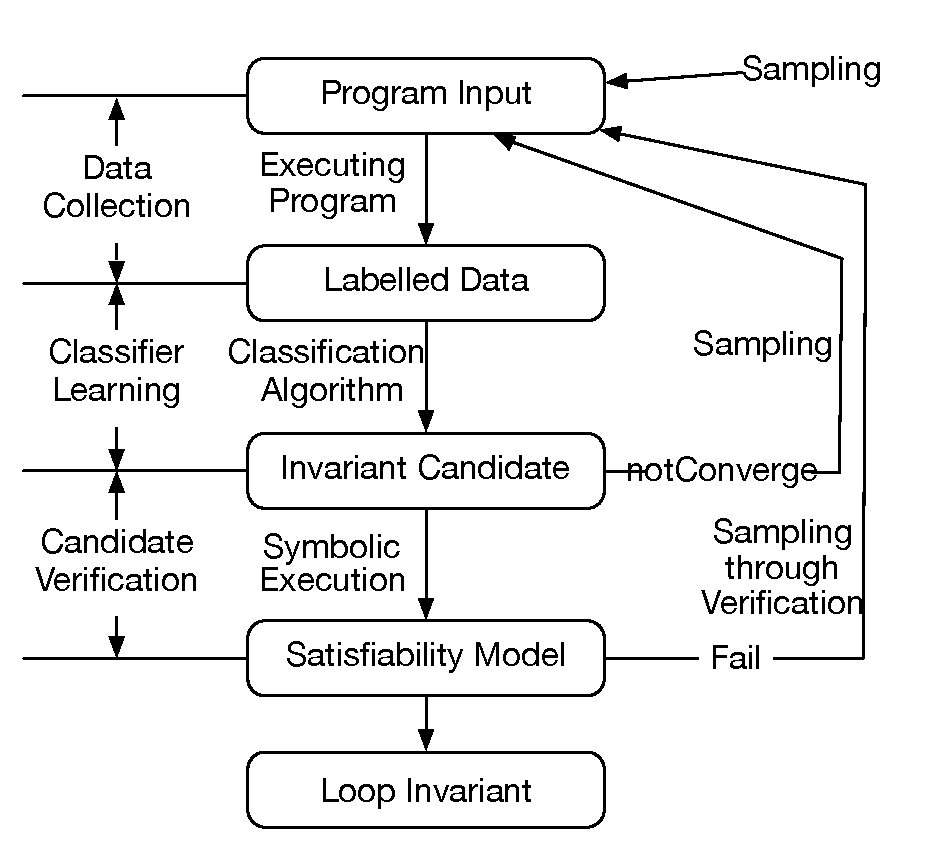
\includegraphics[scale=0.45]{figures/overview.pdf}
    \caption{Loop Invariant Inference Framework Overview}
    \label{fig:overview}
\end{figure}

\begin{figure}[t]
\begin{subfigure}{0.5\textwidth}
    \raggedright
    \vspace{0.5cm}
%% {\scriptsize\begin{verbatim}
%% void P(int x, int y) {
%%     assume(x < y);
%%     while (x < y) {
%%         if (x < 0) x = x + 7;
%%         else x = x + 10;

%%         if (y < 0) y = y - 10;
%%         else y = y + 3;
%%     }
%%     assert(x >= y
%%         && x <= y + 16);
%% }
%% \end{verbatim}}
\vspace{-0.2cm} \[
 \begin{array}{ll}
1 & \code{void~P(int ~x{,} ~int~y)\{} \\
2 & \code{~~~ assume(x~{<}~y);}  \\
3 & \code{~~~ while(x~{<}~y)\{}  \\
4 & \code{~~~ \quad if~(x~{<}~0)~x~{=}~x~{+}~7;}  \\
5 & \code{~~~ \quad else~ x~{=}~x~{+}~10;}\\
6 & \code{~~~ \quad if~(y~{<}~0)~y~{=}~y~{-}~10;} \\
7 & \code{~~~ \quad else~ y~{=}~y~{+}~3;}\\
8 & \code{~~~\}} \\
9 & \code{~~~assert(x~{\geq}~y}\\
10 & \code{~~~\quad \&\&~x~{\leq}~y~{+}~16);}\\
11  & \}
\end{array}
\]
    \vspace{-0.2cm}
    \caption{A sample program}
    \label{fig:running:example:program}
\end{subfigure}%
\begin{subfigure}{.5\textwidth}
      \centering
      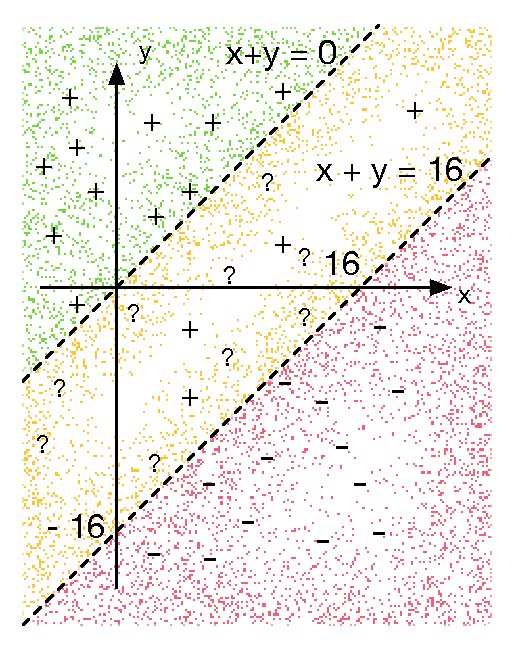
\includegraphics[scale=0.42]{figures/running-sampling.pdf}
      \caption{Sampling}
      \label{fig:running:example:sampling}
\end{subfigure}
\caption{A running example}
\label{fig:running:example}
\end{figure}
%%%sunjun: the two lines should x - y = 0 and x - y = 16.


\begin{example}
An example Hoare triple is shown in Figure~\ref{fig:running:example:program} (where an \code{assume} statement captures the precondition and an \code{assert} statement captures the postcondition). 
The set of variables $V$ contains two integer-type ones: $x$ and $y$. 
For simplicity, we interpret integers in the programs as mathematical integers (i.e., they do not overflow). 
The precondition $\mathit{Pre}$ is $\mathit{x < y}$, which is the same as the loop condition $\mathit{Cond}$.
During each loop iteration, $x$ is increased by $7$ if it is negative (line 4); otherwise, it is increased by $10$ (line 5). 
$y$ is decreased by $10$ if it is negative (line 6); 
otherwise, it is increased by $3$ (line 7). 
The postcondition $\mathit{Post}$ is $\mathit{y \le x \le y + 16}$. 
It is easy to check that the Hoare triple can be proven using a loop invariant $\mathit{Inv}$: $\mathit{x \le y + 16}$. 
In the following, we show how our framework works to learn this loop invariant.
\end{example}
We start with \emph{data collection}. Given the Hoare triple, we first  generate a set of valuations of $V$ randomly. 
% For instance, we can adopt a constraint solver to generate random valuations which satisfy or fail $\mathit{Pre}$ as random samples.
%For each sample $s_0$ (i.e., a variable valuation) $\in V$, 
Then we execute the loop program with $s_0 \in V$ as the initial evaluation and record an evaluation sequence $\{s_0, s_1, s_2, \cdots, s_i, \cdots, s_n\}$ after each iteration of the loop. 
%We donate $s_0$ as the initial evaluation of $s_i$, and $s_n$ as the last evaluation of $s_i$.
%We write $s_i$ as the state after the $i_{th}$ iteration of the loop. %, ~ {0<=i<=n}$
%as a trace $\langle s_0, s_1, \ldots, s_n \rangle$ where $s_n \not \models Cond$. Let $T$ denote the set of traces. We write $s \Rightarrow_T s'$ to denote that there exists a trace $\langle s_0, s_1, \cdots, s, \cdots, s', \cdots, s_n \rangle \in T$.
All the variable valuations $s_i~(0 \leq i \leq n)$ in such an evaluation sequence are divided into the following four sets according to whether $s_0$ satisfies $\mathit{Pre}$ and $s_n$ satisfies $\mathit{Post}$.
Let $\mathit{Inv}$ be any invariant which satisfies condition (1), (2) and (3). 
\begin{itemize}
    \item Set $\mathit{CE}$ contains all the valuations $s_i$ in an evaluation sequence where $\mathit{s_0 \models \mathit{Pre}}$ but $\mathit{s_n \not\models \mathit{Post}}$. We remark that anytime a valuation in $\mathit{CE}$ is identified, a counterexample is found and the Hoare triple is falsified.
    \item Set $\mathit{Positive}$ contains all the valuations $s_i$ in an evaluation where $\mathit{s_0 \models \mathit{Pre}}$ and $\mathit{s_n \models \mathit{Post}}$. In Section~\ref{sec:sampling} we prove that any valuation in $\mathit{Positive}$ must satisfy $\mathit{Inv}$, if $\mathit{Inv}$ exists.
    \item Set $\mathit{Negative}$ contains all the valuations $s_i$ in an evaluation where $\mathit{s_0 \not\models \mathit{Pre}}$ and $\mathit{s_n \not\models \mathit{Post}}$. In Section~\ref{sec:sampling} we prove that any valuation in $\mathit{Negative}$ must fail $\mathit{Inv}$, if $\mathit{Inv}$ exists.
    \item Set $\mathit{NP}$ contains all the valuations which have not appeared in the above three sets. The satisfaction of these valuations to $\mathit{Inv}$ can not be decided according to the current knowledge. So they may or may not satisfy $\mathit{Inv}$.
\end{itemize}
%\begin{itemize}
%    \item Set $\mathit{CE}$ contains the set of valuations which satisfy the precondition and violate the postcondition afterwards. We remark that anytime a valuation in $\mathit{CE}$ is identified, a counterexample is found and the Hoare triple is falsified.
%    \item Set $\mathit{Positive}$ contains the set of valuations which must satisfy $\mathit{Inv}$.
%    \item Set $\mathit{Negative}$ contains the set of valuations which must fail $\mathit{Inv}$.
%    \item Set $\mathit{NP}$ contains the set of valuations which may or may not satisfy $\mathit{Inv}$.
%\end{itemize}
%The exact definition of these sets is in Section~\ref{sec:sampling}.
% Otherwise, because $\mathit{Inv}$ must satisfy (1),(2) and (3), we know that $P_T \subseteq Inv$ and $N_T \cap Inv = \emptyset$. The program states in $NP_T$ may or not may be in $\mathit{Inv}$. If we know that a program state $s \in NP_T$ is in $\mathit{Inv}$, $Body^*(s) \subseteq Inv$.
%
%Each trace is then associated with a pair of boolean labels $(SatPre, SatPost)$
%
%    All of the evaluations in the above trace (referred by its initial evaluation $s_0$)
%    are labelled based on a pair of boolean values
%    $(s_0 \models \mathit{Pre}, s_n \models \mathit{Post})$\footnote{
%        $(\mathit{true}, \mathit{true}) \rightarrow +$,
%        $(\mathit{false}, \mathit{false}) \rightarrow -$
%        and $(\mathit{false}, \mathit{true}) \rightarrow ?$}.
\begin{example}
We illustrate these four sets using the example shown in Figure~\ref{fig:running:example}. Since the Hoare triple is valid, set $\mathit{CE}$ for this example is empty. 
Assume that the following three valuations are randomly sampled initially in our running example: $\mathit{\{x \mapsto 1, y \mapsto 2\}}$, $\mathit{\{x \mapsto 10, y \mapsto 1\}}$ and $\mathit{\{x \mapsto 100, y \mapsto 0\}}$. 
Three sequences of valuations are generated accordingly: $\mathit{\langle \{x \mapsto 1, y \mapsto 2\}, \{x \mapsto 11, y \mapsto 5\} \rangle}$, $\mathit{\langle \{x \mapsto 10, y \mapsto 1\} \rangle}$ and $\mathit{\langle \{x \mapsto 100, y \mapsto 0\} \rangle}$. 
Note that the loop is not executed for the latter two cases. 
As a result, set $\mathit{Negative}$ contains $\mathit{\{x \mapsto 100, y \mapsto 0\}}$; 
set $\mathit{Positive}$ contains $\mathit{\{x \mapsto 1, y \mapsto 2\}}$ and $\mathit{\{x \mapsto 11, y \mapsto 5\}}$; 
and $\mathit{NP}$ contains $\mathit{\{x \mapsto 10, y \mapsto 1\}}$.
\end{example}
Next, we move on to \emph{active learning} to generate candidate invariants based on $\mathit{Positive}$, $\mathit{Negative}$ and $\mathit{NP}$. 
Intuitively, since we know that valuations in $\mathit{Positive}$ must satisfy $\mathit{Inv}$ and valuations in $\mathit{Negative}$ must not satisfy $\mathit{Inv}$, 
a predicate separating the two sets (a.k.a.~a classifier) could be a candidate for $\mathit{Inv}$.
%Formally, a classifier between two sets $P$ and $N$ is a predicate $\phi$ such that $s \models \phi$ for all $s \in P$ and $s \not \models \phi$ for all $s \in N$.
For instance, Figure~\ref{fig:running:example:sampling} shows where the set of valuations 
in $\mathit{Positive}$, $\mathit{Negative}$ and $\mathit{NP}$ locate geographically in a 2-D plane for our running example. %if we consider only the variable valuation before the loop. 
In particular, valuations in $\mathit{Positive}$ are labeled with $+$; % and color green; 
valuations in $\mathit{Negative}$ are labeled with $-$; % and color red; 
and valuations in $\mathit{NP}$ are labeled with ?. % and color yellow. 
%Note that if variable valuations after some iterations of the loop are considered, some of the valuations categorized as $NP$ in Figure~\ref{fig:running:example:sampling} may be in $Positive$ instead as we show in Section~\ref{sec:sampling}.
%, such as $\{x \mapsto 11, y \mapsto 5\} \rangle$.
And there are three areas: a pure positive area with color green, a pure negative area with color red, and a mixed area with color yellow.
The existence of a mixed area is caused by our labeling method which depends much on the observed program valuation sequences.
For example, $\mathit{\{x \mapsto 11, y \mapsto 5\}}$, labeled as `+' in Fig.~\ref{fig:running:example:sampling}, 
could also be labeled as `?' if it only appears in an one execution valuation sequence $\mathit{\langle \{x \mapsto 11, y \mapsto 5\} \rangle}$.
It can be observed the classifier separating $\mathit{Negative}$ from the rest (i.e., $\mathit{x - y \leq 16}$) 
is the loop invariant we are searching for. 
%If we do execute the program with $\{x \mapsto 11, y \mapsto 5\} \rangle$

In order to automatically generate candidate invariants, we apply existing classification techniques to generate classifiers. 
There are however two issues to be solved. The first issue is, with the limited samples in $\mathit{Positive}$ and $\mathit{Negative}$, 
it is unlikely that we can obtain an ``accurate'' classifier. 
For instance, given the above-mentioned set $\mathit{Positive}$ and $\mathit{Negative}$, 
a classifier identified using classification techniques like $\mathit{SVM}$ could be: $\mathit{3x-10y \leq 152}$. %$x+y \leq 50$. 
Although this classifier perfectly separates the current valuations in $\mathit{Positive}$ from $\mathit{Negative}$. 
it is far from our wanted loop invariant and is clearly the result of having limited samples. 
Researchers in the machine learning community have studied extensively on how to overcome the problem of limited samples and one of the remedies is active learning~\cite{DBLP:series/synthesis/2012Settles}. 
Active learning is a semi-supervised machine learning in which a learning algorithm is able to interactively ask for samples which are important in improving a given classifier. 
For instance, active learning for $\mathit{SVM}$ works by repeatedly generating samples on (or nearby) the current classification boundary, adding them into $\mathit{Positive}$ and $\mathit{Negative}$ accordingly and applying $\mathit{SVM}$ to generate new classifiers. 
This process is repeated until the classifier converges. It has been shown that active learning effectively learns an accurate function with fewer samples~\cite{DBLP:conf/icml/SchohnC00}.

\begin{example}
In the above example, given the current classifier $\mathit{3x-10y \leq 152}$, we apply active learning for $\mathit{SVM}$ 
and generate new valuations $\mathit{\{x \mapsto 7, y \mapsto -13\}}$ and $\mathit{\{x \mapsto 14, y \mapsto -11\}}$ %$\{x \mapsto 44, y \mapsto -2\}$ 
by solving the equation $\mathit{3x-10y = 152}$. % (and using an existing $x$ values to figure out the corresponding $y$ value and vice versa). 
Next, we execute the program with these variable valuations, obtain the variable valuation sequences, and add them into $\mathit{CE}$, $\mathit{Positive}$, $\mathit{Negative}$ or $\mathit{NP}$ accordingly. 
With these new samples, a new classifier is then learnt by applying classification algorithms.
\end{example}
The other issue is: how do we handle those valuations in $\mathit{NP}$, which may or may not satisfy $\mathit{Inv}$? 
If we simply ignore them, there may be a gap between $\mathit{Positive}$ and $\mathit{Negative}$ 
and as a result, the learnt classifier may not converge to the invariant we want, even with the help of active learning. 
This is illustrated in Figure~\ref{fig:running:example:sampling}, where $\mathit{NP}$ happens to be located in between $\mathit{Positive}$ and $\mathit{Negative}$. 
Without considering the samples in $\mathit{NP}$, multiple classifiers located in the $\mathit{NP}$ region (e.g., $\mathit{x - y \leq 10}$, or $\mathit{x - y \leq 15}$) may be learnt to perfectly classify $\mathit{Positive}$ and $\mathit{Negative}$. 
Identifying more samples in $\mathit{Positive}$ or $\mathit{Negative}$ may not help to improve the classifier either. 
To overcome the problem, in addition to learn a classifier separating $\mathit{Positive}$ and $\mathit{Negative}$, we learn two additional candidate invariants making use of $\mathit{NP}$: 
one separating $\mathit{Positive}$ from $\mathit{Negative}$ and $\mathit{NP}$ (i.e., assuming valuations in $\mathit{NP}$ fail $\mathit{Inv}$); 
and the other separating $\mathit{Negative}$ from $\mathit{Positive}$ and $\mathit{NP}$ (i.e., assuming valuations in $\mathit{NP}$ satisfy $\mathit{Inv}$). 
We remark that active learning is applied to all three candidates until they converge. 
In our example, if we restrict our learning classifier to linear inequation, 
the classifier separating $\mathit{Positive}$ from $\mathit{Negative}$ and $\mathit{NP}$ would be $\textsc{null}$ (no such a linear classifier); % $\emptyset$, %converge to $\varnothing$ %$\mathit{NULL}$; %x - y \leq 0$; 
and the classifier separating $\mathit{Negative}$ from $\mathit{Positive}$ and $\mathit{NP}$ would converge to $\mathit{x - y \leq 16}$.

After all three candidate invariants converge, we move on to \emph{candidate verification}. 
We check whether any of the candidate invariants satisfies condition (1), (2) and (3). 
In particular, for each candidate invariant $\phi$, we check whether any of the following formula is satisfiable or not using an $\mathit{SMT}$solver~\cite{barrett2009satisfiability,de2008z3}.
\begin{align}
    & \mathit{Pre} \land \neg \phi \label{check:inv:pre} \\
    %% & (s \models \phi \land \mathit{Cond}) \land (\mathit{Body}(s) \not \models \phi) \label{check:inv:loop} \\
     & sp(\phi \land \mathit{Cond}, \mathit{Body}) \land \neg \phi \label{check:inv:loop} \\
    & \phi \land \neg \mathit{Cond} \land \neg \mathit{Post} \label{check:inv:post}
\end{align}
where $\mathit{sp}(\phi,e)$ is the strongest postcondition obtained by
symbolically executing program $e$
starting from precondition $\phi$.
If there is one candidate invariant which fails all the three conditions, we successfully prove the Hoare triple. 
For instance, the candidate invariant $\mathit{x - y \geq 16}$ generated in our example fails all three conditions and we prove the Hoare triple shown in Figure~\ref{fig:running:example:program}. 
If any of condition (4), (5) and (6) is satisfiable, the $\mathit{SMT}$ solver generates a model in the form of a variable valuation, 
and update $\mathit{Positive}$, $\mathit{Negative}$, $\mathit{NP}$ or $\mathit{CE}$ accordingly. % to the execution with these valuations. 
In particular, a counterexample satisfying condition (4) should be added into $\mathit{Positive}$; 
a counterexample satisfying condition (6) may be added into either $\mathit{Negative}$ or $\mathit{CE}$ (depending on whether it satisfies $\mathit{Pre}$). 
Thus, we restart from data collection, i.e., we execute the program with the counterexample valuations, 
collect and add the variable valuations after each iteration of the loop to the four sets accordingly, move on to active learning and so on.

We remark that with the help of active learning, we can often reduce the number of learn-and-check iterations. %, and also the corresponding learning time. 
For our running example, with active learning, usually one iteration of learn-and-check is sufficient to prove the Hoare triple. 
Without active learning, more iterations are often required as shown in Section~\ref{sec:evaluations}. 
In the following sections, we present details on data collection (in Section~\ref{sec:sampling}) and active learning (in Section~\ref{sec:learning}). 
For candidate verification, the standard program verification technique is adopted and thus we only present the relevant implementation details in Section~\ref{sec:evaluations}.

%, with the three sets of valuations $\mathit{Positive}$, $\mathit{Negative}$ and $\mathit{NP}$, we apply active learning techniques to learn a classifier to capture the positive ones from the negative ones   using machine learning algorithms, e.g., SVM derivatives.
%    When the recently learnt classifier converges to the previously learnt ones,
%    we treat it as an invariant candidate and move to the next stage.
%    Otherwise, we apply selective sampling on the recently learnt classifier
%   to add more samples to $S_{\mathit{in}}$.
%    When a sample cannot be classified using a certain classification model,
%    we try other alternative models in a sequential order.
%    \LL{We prove the termination of the \emph{active learning} stage if such an invariant exists.}



%    In the \textbf{Invariant Verification} stage (see Section~\ref{sec:verification}),
%    we check the correctness of the invariant candidate.
%    First, we check condition (\ref{inv:pre}) and condition (\ref{inv:post}) with the candidate.
%    Then, we verify the condition (\ref{inv:loop})
%    based on all of the program execution traces of $\mathit{Body}$ using symbolic execution~\cite{}.
%    The above conditions are checked by SMT~\cite{barrett2009satisfiability} solvers in this work.
%    If all of the above conditions are satisfied,
%    we claim the correctness of $P$ with its loop invariant.
%    Otherwise, we add the counter-example from SMT Solving to $S_{\mathit{in}}$
%    and restart from the \emph{data collection} stage.

%The overall algorithm is shown in Algorithm~\ref{alg:overall}.
%\section {Overall Algorithm}
%\label{sec:overall}
% \LL{Do not put the algorithm here. It contains lots of notations undefined.}
% The overall algorithm is presented in Figure~\ref{alg:overall}.
% \begin{algorithm}[!h]
% \SetAlgoVlined
% \Indm
% \KwIn{$Pre$, $Cond$, $Body$, $Post$}
% \KwOut{an invariant which completes the proof or a counter-example}
% \Indp
% let $S$ be \textsc{Null}\;
% \While{true} {
%     add Samples into $S$\;
%     test the program for each sample in $S$\;
%     \If {a state $s$ in $\mathcal{S}^x$ is identified} {
%         \Return $s$ as a counterexample;
%     }
%     let $\mathcal{S}^+$, $\mathcal{S}^-$ and $\mathcal{S}^\rightarrow$ be respective sets accordingly\;
%     let $\mathcal{C}$ = activeLearning($\mathcal{S}^+$, $\mathcal{S}^-$, $\mathcal{S}^\rightarrow$)\;
%     Extract path constraints $\textsc{Pc}$ based on (1)(2)(3)\;
%     \For {each $pc$ in $\textsc{Pc}$} {
%         \If { $pc$ is not satisfied} {
%             add the counter-example into $S$\;
%             continue\;
%         }
%     }
%     \Return $\mathcal{C}$ as the proof;
% }
% \caption{Algorithm $overall$}
% \label{alg:overall}
% \end{algorithm}
%
% \begin{theorem}
% Algorithm $overall$ always eventually terminates and it is correct. \hfill \qed
% \end{theorem}



\section{The Overall Approach}
\label{sec:overview}
Loop invariant generation using a guess-and-check approach is an iterative process of \emph{data collection}, \emph{guessing} (i.e., classification in this work) and checking (i.e., verification of the invariant candidate).
%The overall workflow is shown in the Figure~\ref{fig:overview}.
In the following, we present how our approach works step-by-step and illustrate each step with simple examples.

\begin{example}
A few example Hoare triples are shown in Figure~\ref{fig:running:example}, where an \code{assume} statement captures the precondition and an \code{assert} statement captures the postcondition.
The set of variables $V$ for each program contains two integer-type ones: $x$ and $y$. For simplicity, we write $(a, b)$ where $a$ and $b$ are integer constants to denote the  evaluation $\{x \mapsto a, y \mapsto b\}$. Further, we interpret integers in the programs as mathematical integers (i.e., they do not overflow).
%During each loop iteration, $x$ is increased by $7$ if it is negative (line 4); otherwise, it is increased by $10$ (line 5).
%$y$ is decreased by $10$ if it is negative (line 6);
%otherwise, it is increased by $3$ (line 7).
%The postcondition $Post$ is $y \le x \le y + 16$.
One example invariant which can be used to prove the Hoare triple is shown for each program. For instance, the Hoare triple shown in Figure~\ref{fig:running:example:programa} can be proven using a loop invariant: $x \le y + 16$, whereas conjunctive or disjunctive invariants are necessary to prove the other Hoare triples. In the following, we show how we generate loop invariants for proving these Hoare triples.
\end{example}
\noindent The overall approach is shown as Algorithm~\ref{alg:active}. We start with randomly generating a set of valuations of $V$, denoted as $SP$, at line 1 (a.k.a.~random sampling). Random sampling provides us the initial set of samples to learn the very first candidate for the loop invariant.
In this work, we have two ways to generate random samples. One is that we generate random values for each variable in $V$ based on its domain,
assuming a uniform probabilistic distribution over all values in its domain.
The other is that we apply an SMT solver~\cite{barrett2009satisfiability,de2008z3} to generate valuations that satisfy $Pre$
as well as those that fail $Pre$. These two ways are complementary.
On one hand, without using a solver, we may not be able to generate valuations which satisfy $Pre$ if $Pre$ is very restrictive
(or fail $Pre$ if the negation of $Pre$ is very restrictive). On the other hand, using a solver often generates biased valuations. %We remark that the cost of generating a random sample is often negligible.

\begin{figure}[t]
\begin{subfigure}{0.5\textwidth}
    \raggedright
\[
 \begin{array}{ll}
1 & \code{~~~ assume(x~{<}~y);}  \\
2 & \code{~~~ while(x~{<}~y)\{}  \\
3 & \code{~~~ \quad if~(x~{<}~0)~x~{=}~x~{+}~7;}  \\
4 & \code{~~~ \quad else~ x~{=}~x~{+}~10;}\\
5 & \code{~~~ \quad if~(y~{<}~0)~y~{=}~y~{-}~10;} \\
6 & \code{~~~ \quad else~ y~{=}~y~{+}~3;}\\
7 & \code{~~~\}} \\
8 & \code{~~~assert(y~{\leq}~x~{\leq}~y~{+}~16);}
\end{array}
\]
\vspace{-2mm}
    \caption{Invariant: $x \le y + 16$}
    \label{fig:running:example:programa}
\end{subfigure}%
\begin{subfigure}{.5\textwidth}
\[
 \begin{array}{ll}
1 & \code{~~~ assume(x==1 {\land} y==0);}  \\
2 & \code{~~~ while(*)\{}  \\
3 & \code{~~~ \quad x = x + y;}  \\
4 & \code{~~~ \quad y = y + 1;}\\
5 & \code{~~~\}} \\
6 & \code{~~~assert(y~{\geq}~x);}
\end{array}
\]
    \caption{Invariant: $y \geq 0 \land y \geq x$}
    \label{fig:running:example:programb}
\end{subfigure}
   \begin{subfigure}{0.5\textwidth}
    \raggedright
     \vspace{0.3cm}
        \[
      \begin{array}{ll}
      1 & \code{assume(x~{>}~0~ {||} ~y~{>}~0);}  \\
      2 & \code{while(x~{+}~y~{\le}-2)\{}  \\
      3 & \code{\quad if~(x~{>}~0) ~~~x{++};}  \\
      4 & \code{\quad else~ ~~~y = y + 1;}\\
      5 & \code{\}} \\
      6 & \code{assert(x~{>}~0~ {||} ~y~{>}~0);}\\
      \end{array}
    \]
    \caption{Invariant: $x > 0 \lor y > 0$}
    \label{fig:running:example:programc}
   \end{subfigure}%
   \begin{subfigure}{0.5\textwidth}
     \vspace{0.3cm}
      \[
      \begin{array}{ll}
      1 & \code{assume(x < 0)} \\
      2 & \code{while(x < 0)\{}  \\
      3 & \code{~~~ \quad x = x + y;}  \\
      4 & \code{~~~ \quad y++; \}}  \\
      5 & \code{\}} \\
      6 & \code{assert();}
      \end{array}
    \]
    \caption{Invariant: $x < 0 \lor y > 0$}
    \label{fig:running:example:programd}
   \end{subfigure}
\caption{Example programs}
\label{fig:running:example}
\end{figure}

Next, for any valuation $s$ in $SP$, we execute the program starting with initial variable valuation $s$ and record the valuation of $V$ after each iteration of the loop. We write $s \Rightarrow s'$ to denote that there exists $i \geq 0$ such that $s' = Body^i(s)$ and $Body^k(s) \in Cond$ for all $k \in [0, i)$. That is, if we start with valuation $s$, we obtain $s'$ after some number of iterations. At line 3 of Algorithm~\ref{alg:active}, we add all such valuations $s'$ into $SP$. Next, we categorize $SP$ into the four disjoint sets: $CE$, $Positive$, $Negative$ and $NP$. Intuitively, $CE$ contains counterexamples which disprove the Hoare triple; $Positive$ contains those valuations of $V$ which we know must satisfy any loop invariant which proves the Hoare triple; $Negative$ contains those valuations of $V$ which we know must not satisfy any loop invariant which proves the Hoare triple; and $NP$ contains the rest. Formally,
\[
CE(SP) = \{s \in SP |s \in Pre \land~\exists s'.~s \Rightarrow s' \land s' \not \in Cond \land s' \not \in Post\} \]
A valuation in $CE(SP)$ satisfies $Pre$ and becomes a valuation $s'$ which fails $Post$ when the loop terminates. If $CE(SP)$ is non-empty, the Hoare triple is disproved.
%\begin{align*}
% \mathit{Positive}(\mathit{SP}) = & \{s | \exists s_0 \in SP.~\exists s'.~s_0 \Rightarrow s' \Rightarrow s \Rightarrow s_n \land \\
%     & ~~~~~~s' \models \mathit{Pre} \land s_n \not \models Cond \land s_n \models \mathit{Post}\}
%\end{align*}
%\begin{align*}
\begin{align*}
Positive(SP) = & \{s \in SP | \exists s_0,s_1: SP. \\
& ~~~~~~ s_0 \in Pre \land s_0 \Rightarrow s \Rightarrow s_1 \land s_1 \not \in Cond \land s_1 \in Post\}
\end{align*}
$Positive(SP)$ contains a valuation $s$ if there exists a valuation $s_0$ in $SP$ which satisfies $Pre$ and becomes $s$ after zero or more iterations. Furthermore, $s$ subsequently becomes $s'$ which satisfies $Post$ when the loop terminates. Let $Inv$ be any loop invariant which proves the Hoare triple. Because $s_0 \in Pre$, $s_0 \in Inv$ since $Inv$ satisfies condition (1). Since $Inv$ satisfies condition (2) and $Body(s_0) \in Inv$ if $Body(s_0) \in Cond$. By a simple induction, we prove $s \in Inv$.
\begin{align*}
    Negative(SP) = & \{s \in SP | s \not \in Pre \land \exists s'. \\
    & ~~~~~~s \Rightarrow s' \land s' \not \in Cond \land s' \not \in Post\}
\end{align*}
$Negative(SP)$ is the set of valuations which violates $Pre$ and becomes a valuation $s'$ which violates $Post$ when the loop terminates. We show that $s \not \in Inv$ for all $Inv$ satisfying condition (1), (2) and (3). Assume that $s \in Inv$, by condition (2), $s'$ must satisfy $Inv$ through a simple induction. By condition (3), $s'$ must satisfy $Post$, which contradicts the definition of $Negative(SP)$.
\[    NP(SP) = SP - CE(SP) - Positive(SP) - Negative(SP)
\]
$NP(SP)$ contains the rest of the samples. We remark that a valuation $s$ in $NP(SP)$ may or may not satisfy an invariant $Inv$ which satisfies condition (1), (2) and (3).

\begin{algorithm}[t]
\SetAlgoVlined
\Indm
\Indp
let $SP$ be a set of randomly generated valuations of $V$\;
\While{not time out} {
    add all valuations $s'$ such that $s \Rightarrow s'$ for some $s \in SP$ into $SP$\;
    call $actL(SP)$ to generate a candidate invariant\;
    return ``proved'' if the program is verified with $\phi$ otherwise add the counterexample into $SP$\;
}
\caption{Algorithm $zilu()$}
\label{alg:active}
\end{algorithm}

\begin{example} \label{example2}
Take the program shown in Figure~\ref{fig:running:example:programa}. Assume that the following three valuations are randomly generated:
$(1, 2)$, $(10, 1)$ and $(100, 0)$ at line 1. Three sequences of valuations are generated after executing the program with these three valuations: $\langle (1, 2), (11, 5) \rangle$, $\langle (10, 1) \rangle$ and $\langle (100, 0) \rangle$.
Note that the loop is skipped entirely for the latter two cases. After categorization, set $CE(SP)$ is empty; $Positive(SP)$ is $\{(1, 2),(11, 5)\}$; $Negative(SP)$ is $\{(100, 0)\}$; and $NP(SP)$ is $\{(10, 1)\}$.
\end{example}
After obtaining the samples and labeling them as discussed above, method $actL(SP)$ at line 4 in Algorithm~\ref{alg:active} is invoked to generate a candidate invariant $\phi$. We leave the details on how candidate invariants are generated in Section~\ref{sec:classifierlearning}, which is our main contribution in this work. Once a candidate is identified, we move on to check whether $\phi$ satisfies condition (1), (2) and (3) at line 5. In particular, we check whether any of the following constraints is satisfiable or not using an $SMT$ solver~\cite{barrett2009satisfiability,de2008z3}.
\begin{align}
    & \mathit{Pre} \land \neg \phi \label{check:inv:pre} \\
     & sp(\phi \land Cond, Body) \land \neg \phi \label{check:inv:loop} \\
    & \phi \land \neg Cond \land \neg Post \label{check:inv:post}
\end{align}
where $sp(\phi \land Cond,Body)$ is the strongest postcondition obtained by symbolically executing program $Body$ starting from precondition $\phi \land Cond$~\cite{DBLP:journals/cacm/Dijkstra75}. If all the three constraints are unsatisfiable, we successfully prove the Hoare triple with loop invariant $\phi$. If any of the constraints is satisfiable, a model in the form of a variable valuation is generated, which is then added to $SP$ as a new sample. Afterwards, we restart from line 1, i.e., we execute the program with the counterexample valuations, collect and add the variable valuations after each iteration of the loop to the four categories accordingly, move on to active learning and so on.
\begin{example}
For the example shown in Figure~\ref{fig:running:example:programa}, a candidate invariant which is automatically learned is $x - y \geq 16$. It is easy to check that this candidate satisfies all the three conditions and thus the Hoare triple shown in Figure~\ref{fig:running:example:programa} is proved. For the example shown in Figure~\ref{fig:running:example:programc}, a candidate invariant returned by method $actL(SP)$ is as follows.
\[
246 + 23x + 3y \geq 0 \lor -174 - 7x + 36y \geq 0
\]
A counterexample $(-11, 1)$ is generated when we check the satisfiability of (4), which is then used to generate a new candidate. After 3 iterations of guess-and-check, the following invariant is generated.
\[
33 - 2x + 2y \geq 0 \lor 5 - 2x + 2y \geq 0 \lor 23 - 2x + 2y \geq 0
\] 
Unexpectedly, this invariant turns out to be one which is strong enough to prove the Hoare triple.
\end{example}



\section{Our Approach: Classification and Active Learning}
\label{sec:classifierlearning}
In this section, we present details on how candidate loop invariants are generated. Algorithm~\ref{classification} shows how $actL(SP)$ is implemented in general, i.e., it iteratively generates a candidate through classification (at line 3) and improves it through active learning (at line 5) until a fixed point is reached. Note that any time a counterexample is identified (at line 2), our approach exits and reports that the Hoare triple is disproved.

\begin{algorithm}[t]
\SetAlgoVlined
\Indm
\Indp
\While{true} {
    if ($CE(SP)$ is not empty) { exit and report ``disproved''; } \\
    let $\phi$ be a set of candidates generated by $classify(SP)$\;
%    let $c$ be $classify(Positive(SP), Negative(SP))$\;
%    //alternatively: let $c$ be $classify(Positive(SP), Negative(SP) \cup NP(SP))$; \\
%    //alternatively: let $c$ be $classify(Positive(SP) \cup NP(SP), Negative(SP))$; \\
    if ($\phi$ is the same as last iteration){ return $\phi$; } \\
    add $selectiveSampling(\phi)$ into $SP$\;
    add all valuations $s'$ such that $s \Rightarrow s'$ for some $s \in SP$ into SP\;
}
\caption{Algorithm $actL(SP)$}
\label{classification}
\end{algorithm}

The method call $classify(SP)$ at line 3 in Algorithm~\ref{classification} generates a candidate invariant based in classification. Intuitively, since we know that valuations in $Positive(SP)$ must satisfy $Inv$ and valuations in $Negative(SP)$ must not satisfy $Inv$, a predicate separating the two sets (a.k.a.~a classifier) may be a candidate invariant. In the following, we fix two disjoint sets of samples $P$ and $N$ and discuss how to automatically generate classifiers separating $P$ and $N$. For now, $P$ can be understood as $Positive(SP)$ and $N$ can be understood as $Negative(SP)$. We discuss alternatives in Section~\ref{alternative}.

To automatically generate classifiers separating $P$ and $N$, we apply existing classification techniques. There are many classification algorithms, e.g., perceptron~\cite{perceptron}, decision tree~\cite{quinlan1986induction} and Support Vector Machine (SVM)~\cite{svm:original}.
In our approach, the classification algorithms must generate perfect classifiers. Formally, a perfect classifier $\phi$ for $P$ and $N$ is a predicate such that $s \in \phi$ for all $s \in P$ and $s \not \in \phi$ for all $s \in Negative$. Furthermore, the classification algorithms must generate classifiers which are human-interpretable or can be handled by existing program verification techniques.
In the following, we show how to adopt existing algorithms to generate candidate invariants based on SVM in Section~\ref{existing}. Next, we present an approach to generate disjunctive invariants in Section~\ref{disjunctive}. Lastly, we show how to improve all these candidates systematically through active learning in Section~\ref{active}.

\subsection{Linear and Polynomial Classifiers} \label{existing}
In~\cite{sharma2012interpolants}, the authors propose to use SVM to generate candidate invariants. SVM is a supervised machine learning algorithm for classification and regression analysis~\cite{svm:original}.
In general, the binary classification functionality of SVM works as follows. Given $P$ and $N$, SVM generates a perfect classifier to separate them if there is any.
%In the following, we write $svm(P, N)$ to denote the function which returns a perfect linear classifier for $P$ and $N$ if there is any; or returns $\textsc{null}$ otherwise.
We refer the readers to~\cite{svm:smo} for details on how the classifier is computed. In this work, we always choose the \textit{optimal margin classifier} if possible. Intuitively, the optimal margin classifier could be seen as the strongest witness why $P$ and $N$ are different.
SVM by default learns classifiers in the form of a linear inequality, i.e., a half space in the form of $c_1x_1 + c_2x_2 + \cdots \geq k$ where $x_i$ are variables in $V$ whereas $c_i$ are constants.

In practice, linear classifiers may not be sufficient in proving certain Hoare triples and thus more expressive invariants are necessary. We can easily extend SVM to learn polynomial classifiers. Given $P$ and $N$ as well as a maximum degree $d$ of the polynomial classifier, we can systematically map all the samples in $P$ (similarly $N$) to a set of samples $P'$ (similarly $N'$) in a high dimensional space by expanding each sample with terms with degree up to $d$. For instance, assume that the maximum degree is 2, the sample valuation $\{ x \mapsto 2, y \mapsto 1\}$ in $P$ is mapped to $\{x \mapsto 2, y \mapsto 1, x^2 \mapsto 4, xy \mapsto 2, y^2 \mapsto 1\}$.
SVM is then applied to learn a perfect linear classifier for $P'$ and $N'$. Mathematically, a linear classifier in the high dimensional space is the same as a polynomial classifier in the original space~\cite{svm:kernel}.
We remark that the size of each sample in $P'$ or $N'$ grows rapidly with the increase of the degree and thus the above method is often limited to polynomial classifiers with relatively low degree.

A polynomial classifier can represent classifiers in the form of disjunctive or conjunctive linear inequalities. For instance, the classifier $(x \ge d_0) \wedge (x \le d_1)\big) \vee (x \ge d_2)$
where $d_0 < d_1 < d_2$ are constants can be represented equivalently as the following polynomial inequality.
\[
x^3 + (d_0d_1 + d_0d_2 + d_1d_2)x^2 - (d_0 + d_1 + d_2)x - d_0d_1d_2 \geq 0
\]
However, it is not always possible, i.e., some conjunctive or disjunctive linear inequalities cannot be expressed in the form of a polynomial classifier. One simple example is: $x \ge 0 \land y \ge 0$.

In~\cite{sharma2012interpolants}, an algorithm for learning conjunctive classifiers is proposed. The idea is to pick one sample $s$ from $N$ each time and identify a classifier $\phi_i$ (which could be a linear or polynomial one) to separate $P$ and $\{s\}$, remove all samples from $N$ which can be correctly classified by $\phi_i$, and then repeat the process until $N$ becomes empty. The conjunction of all the classifiers is then a perfect classifier. We refer the readers to~\cite{sharma2012interpolants} for details of the algorithm. %This approach however may learn a classifier with many clauses. In the worse case, if each classifier $\phi_i$ only classifies the one sample $s$, the returned classifier would conjunct as many clauses as the number of samples in $N$.

\subsection{Disjunctive Classifiers} \label{disjunctive}
It is challenging in general to automatically generate disjunctive invariants~\cite{DBLP:conf/cav/SharmaDDA11,DBLP:conf/pldi/GulwaniSV08}, whereas certain Hoare triples can only be proved with disjunctive invariants. Two examples are shown in Figure~\ref{fig:running:example}(b) and Figure~\ref{fig:running:example}(d). In the following, we show how to learn disjunctive invariants through a path-sensitive classification. Our observation is that disjunctive invariants are relevant often because the program contains branching commands (\code{if}, \code{while}). %% branches.
 For instance, proving the Hoare triple shown on the left of Figure~\ref{fig:running:example}(b) requires a disjunctive loop invariant, which is largely due to the conditional branch at line 3. Based on this observation, we apply the following approach to learn disjunctive invariants.

Assume that the loop body $Body$ contains a finite set of control locations. For instance, the loop in the first program in Figure~\ref{fig:running:example}(b) has four locations: line 3, 4, 5 and 6. Given a valuation of $V$, say $s$, we write $visit(s)$ to be the set of control location which is visited if we execute the program with initial variable valuation $s$ during the first iteration of the loop. For instance, given the program in Figure~\ref{fig:running:example}(b), $visit(\{x \mapsto 0, y \mapsto -3\})$ returns $\{3,6\}$. If $s$ does not satisfy the loop condition $Cond$, $visit(s)$ returns an empty set. We first partition $P$ into a set of disjoint partitions such that all valuations in the same partition $P_i$ visits the same set of control locations. Next, we apply the above-mentioned classification algorithms to learn a classifier for each partition, i.e., we learn a classifier $\phi_i$ for partition $i$ separating $P_i$ from $N$.
Since any sample in $P_i$ satisfies $\phi_i$ and any sample in $N$ does not satisfies, the disjunction $\bigvee_i \phi_i$ is a perfect classifier separating $P$ from $N$. Note that since $P_i$ could be a conjunctive predicate if we apply the algorithm in~\cite{sharma2012interpolants}, we can learn candidate invariants in the form of disjunctions of conjunctions of linear or polynomial predicates.

\begin{example}
Given the program shown in Figure~\ref{fig:running:example}(b), if $P$ is set to be $Positive(SP)$, we have three partitions. The first one contains all valuations $s$ with $visits(s)$ being $\{3,4,5\}$; the second one contains all valuations $s$ with $visits(s)$ being $\{3,6\}$ and the last one contains all valuations $s$ with $visits(s)$ being the empty set. Intuitively, we can see that the classifiers which could be learned if we have every valuation of $V$ for these three partitions should be: $x > 0$, $y>0$ and $x+y > -2$ respectively. The last one is equivalent to the negation of the loop condition because all valuations satisfying $Pre$ and skipping the loop satisfy $Post$. The loop candidate is then: $x > 0 \lor y > 0 \lor x+y>-2$, which satisfies condition (1), (2) and (3) and thus proves the Hoare triple.

Though the program shown in Figure~\ref{fig:running:example}(d) contains no \code{if} command,
it contains a conditional branch of the \code{while} command. %% we show that we can nonetheless
In the following, we show how to apply this approach to learn a necessarily disjunctive loop invariant.
 Variable valuations in $Positive(SP)$ for the example can be partitioned into two: one containing those visit line 3 and 4, the other containing those skipping the loop. Note that a valuation $s$ is in $Negative(SP)$ only if $s \in (y\leq 0 \land x \geq 0)$. If we have every valuation of $V$ for these two partitions, a classifier we could learn for the former partition is $x < 0$ (i.e., as long as a valuation must satisfy the invariant if it enters the loop) and the classifier we learn for the latter partition is $y > 0$. As a result, we learn the candidate invariant: $x < 0 \lor y > 0$, which proves the Hoare triple.

We remark that in the above discussion, we assume that we can obtain every variable valuation, which is often infeasible in practice as there are too many of them. In the following subsection, we aim to solve this problem.
\end{example}

%\begin{figure}[t]
%   \begin{subfigure}{0.5\textwidth}
%    \raggedright
%    % \vspace{0.5cm}
%    \[
%      \begin{array}{ll}
%      1 & \code{assume(x~{>}~0~ {||} ~y~{>}~0);}  \\
%      2 & \code{while(x~{+}~y~{\le}-2)\{}  \\
%      3 & \code{\quad if~(x~{>}~0) ~~~x{++};}  \\
%      4 & \code{\quad else~ ~~~y{++};}\\
%      5 & \code{\}} \\
%      6 & \code{assert(x~{>}~0~ {||} ~y~{>}~0);}\\
%      \end{array}
%    \]
%%     \caption{A sample program}
%%     \label{fig:sl1:example:program}
%   \end{subfigure}%
%   \begin{subfigure}{0.5\textwidth}
%      \[
%      \begin{array}{ll}
%      1 & \code{assume(x < 0)} \\
%      2 & \code{while(x < 0)\{}  \\
%      3 & \code{~~~ \quad x = x + y;}  \\
%      4 & \code{~~~ \quad y++; \}}  \\
%      5 & \code{\}} \\
%      6 & \code{assert(y>0);}
%      \end{array}
%    \]
%   \end{subfigure}
%\caption{Sample programs with disjunctive loop invariants}
%\label{fig:disjunctive:example}
%\end{figure}

%\subsubsection{Disjunctive Invariants for Loop Body with 2 Branches}
%Formally, the Hoare triple for any loop body with two branches can be expressed in the following form on the left side.
%% where $\mathit{Pre}$ is named the precondition while $\mathit{Post}$ is named the postcondition, and $\mathit{Cond}$ is named the loop condition.
%In the loop body, $\mathit{C_1}$ guards the first branch $\mathit{Body_1}$, while $\mathit{\neg C_1}$ guards the other branch $\mathit{Body_2}$.
%\begin{align}
%&\{\mathit{Pre}\} && \emph{Pre} \Rightarrow \emph{$Inv_1$} \vee \emph{$Inv_2$} \label{ext:inv:pre}\\
%&\mathit{while} (\mathit{Cond}) \{ && \\
%&~~~~~~~~\mathit{if} (\mathit{C_1}) ~~\{ \mathit{Body_1} \} && \{(\emph{$Inv_1$} \vee \emph{$Inv_2$}) \wedge Cond \wedge C_1\} Body_1 \{\emph{$Inv_1$}\} \label{ext:inv:loop:b1}\\
%&~~~~~~~~\mathit{else} ~~\{ \mathit{Body_2} \} && \{(\emph{$Inv_1$} \vee \emph{$Inv_2$}) \wedge Cond \wedge \neg C_1\} Body_2 \{\emph{$Inv_2$}\} \label{ext:inv:loop:b2}\\
%&\} && \\
%&\{\mathit{Post}\} && (\emph{$Inv_1$} \vee \emph{$Inv_2$}) \wedge \neg Cond \Rightarrow \emph{Post} \label{ext:inv:post}
%\end{align}
%If the Hoare triple is valid, $Inv_1 \vee Inv_2$ that satisfies the conditions on the right side is defined as the loop invariant for the program,
%in which $Inv_1$ and $Inv_2$ are invariants for corresponding branches.
%% For example, $Inv_1$ is the branch invariant for the first branch as it is evaluated true after execution of $Body_1$ as shown in~\ref{sl1:ext:inv:loop:b1}.
%In our context, branch invariant is a property that always holds for the given branches.
%
%% in which $Inv_1$ and $Inv_2$ are named as branch invariants for the two branches.
%%Assume the invariant for the loop is in the form of $Inv_1 \vee Inv_2$.
%%Note that, any invariant $i$ can be converted to this form by linking itself with disjunction operator, such as $i \vee i$.
%%If there are $Inv_1$ and $Inv_2$ satisfy the following conditions,
%%then $Inv_1 \vee Inv_2$ is a loop invariant for the original program.
%
%In the following, we prove that for loop programs with 2 branches,
%the above definition of loop invariant is equivalent with the previous invariant definition.
%Therefore, we need to prove such $Inv_1 \vee Inv_2$ is a valid loop invariant for the loop program,
%and any loop invariant for the program can be written as $Inv_1 \vee Inv_2$, where $Inv_1$ and $Inv_2$ are branch invariants.
%
%% \begin{theorem}
%% Algorithm~\ref{ta_feasiblefuncwithsim} is sound and complete.
%% \vspace{-1mm}
%% \end{theorem}
%% \noindent \textbf{Proof:} As we discussed the difference between Algorithm~\ref{ta_feasiblefuncwithsim} and Algorithm~\ref{ta_feasiblefunc}, given a transition system $\mathcal{L}$ with a set of initial states $Init$, the transition relation $Tr$ and a set of \buchi conditions $J$, while $IsEmpty(Init, Tr, J)$ is checking the emptiness of $\mathcal{L}$, $IsEmpty_{sim}(Init, Tr, J)$ is actually checking the emptiness of the transition system $\mathcal{L'}$. Thus, the correctness of Algorithm~\ref{ta_feasiblefuncwithsim} is obtained based on Theorem~\ref{theoremofabstractedsystem}.\hfill \qed \\
%
%\begin{theorem}
%\label{thm:disjunctive:is:invariant}
%	$Inv_1 \vee Inv_2$ is a loop invariant for the given loop program.
%\end{theorem}
%
%\noindent \textbf{Proof:} In order to prove $Inv_1 \vee Inv_2$ is a loop invariant for the program,
%we need to show it satisfies all the three conditions~\ref{org:inv:pre}, ~\ref{org:inv:loop} and ~\ref{org:inv:post}.
%
%By simply substituting $Inv$ with  $Inv_1 \vee Inv_2$,
%we can see $Inv_1 \vee Inv_2$ satisfies condition~\ref{org:inv:pre} and ~\ref{org:inv:post}.
%For condition~\ref{org:inv:loop},
%as the valuations obtained through the two branches satisfy $Inv_1$ and $Inv_2$ respectively,
%the valuations for the loop body must satisfy $Inv_1 \vee Inv_2$ naturally.
%Thus, by combining the condition~\ref{ext:inv:loop:b1} and~\ref{ext:inv:loop:b2},
%\begin{align*}
%&\{(Inv_1 \vee Inv_2) \wedge Cond \wedge C_1\} Body_1 \{Inv_1\} \\
%&\{(Inv_1 \vee Inv_2) \wedge Cond \wedge \neg C_1\} Body_2 \{Inv_2\}
%\end{align*}
%we can get $\{(Inv_1 \vee Inv_2) \wedge Cond\}~if (C1)~{Body_1}~else~{Body_2}~\{Inv_1 \vee Inv_2\}$,
%which satisfies the second condition in loop invariant definition.
%
%Therefore, $Inv_1 \vee Inv_2$ is a loop invariant for the given loop program. %\hfill \qed \\
%
%\begin{theorem}
%\label{thm:invariant:is:disjunctive}
%	Any invariant $Inv$ for the given loop program with branches can be expressed in the form of $Inv_1 \vee Inv_2$.
%\end{theorem}
%
%\noindent \textbf{Proof:} If $Inv$ is a loop invariant for the given loop program,
%then $Inv$ satisfies the three conditions ~\ref{org:inv:pre}, ~\ref{org:inv:loop} and ~\ref{org:inv:post}.
%As $Inv = Inv \vee Inv$ always holds, we assign $Inv_1 = Inv$ and $Inv_2 = Inv$.
%Then the three conditions can be easily verified. %\hfill \qed \\
%
%\subsection{Disjunctive Invariants for Loop Body with $\emph{n}$ Branches}
%For the loop body with $n$ branches and valuations for each branch satisfy $Inv_1$, $Inv_2$, $\cdots$, $Inv_n$ respectively,
%it is similar to prove the loop invariant defined as $Inv_1 \vee Inv_2 \vee \cdots \vee Inv_n$ is equivalent to the invariant defined before,
%which means we can apply same technique to combine all the branch invariants together as the candidate loop invariant.
%
%\subsubsection{Disjunctive Invariant Learning Algorithm}
%Assume a Hoare triple that there are 2 branches in the loop body is given,
%and thus our invariants can be written as $(Inv_1 \vee Inv_2 \vee \cdots \vee Inv_n)$.
%Without loss of generality, we take branch $B_i~(1 \le i \le n)$ , whose branch invariant $Inv_i$ accordingly, as an example.
%We build a new set $\mathit{Positive\_B_i}$ by extracting the valuations in $\mathit{Positive}$ which are obtained after passing branch $B_i$.
%According to definition in~\ref{ext:inv:loop:b1} and \ref{ext:inv:loop:b2},
%valuations in $\mathit{Positive\_B_i}$ must satisfy $Inv_i$.
%For any valuation $s \in \mathit{Negative}$,
%we can infer $s \not \models Inv_i$ since $s \not \models Inv_1 \vee Inv_2 \vee \cdots \vee Inv_n$.
%Therefore, all the valuation in $\mathit{Negative}$ fails any branch invariant $Inv_i $.
%
%As a result, we can apply Algorithm~\ref{alg:polynomialSVM} on set $\mathit{Positive\_B_i}$ against set $\mathit{Negative}$ to learn a classifier as the candidate for $Inv_i$.
%Similar procedures are adapted for other branches and the approach can generate an invariant candidate by combining all the classifiers.
%
%\paragraph{Example}
%In the following, we use an illustrative example to show how our framework works on disjunctive invariant learning.
%
%% can apply the primary SVM
%\begin{figure}[t]
%  % \begin{subfigure}{0.5\textwidth}
%    \raggedright
%    % \vspace{0.5cm}
%     \vspace{-0.2cm} \[
%      \begin{array}{ll}
%      1 & \code{void~foo(int ~x{,} ~int~y)\{} \\
%      2 & \code{~~~ assume(x~{>}~0~ {||} ~y~{>}~0);}  \\
%      3 & \code{~~~ while(x~{+}~y~{\le}-2)\{}  \\
%      4 & \code{~~~ \quad if~(x~{>}~0) ~~~x{++};}  \\
%      5 & \code{~~~ \quad else~ ~~~y{++};}\\
%      6 & \code{~~~\}} \\
%      7 & \code{~~~assert(x~{>}~0~ {||} ~y~{>}~0);}\\
%      8 & \}
%      \end{array}
%    \]
%  %   \vspace{-0.2cm}
%  %   \caption{A sample program}
%  %   \label{fig:sl1:example:program}
%  % \end{subfigure}%
%  % \begin{subfigure}{0.5\textwidth}
%  %   \centering
%  %   \includegraphics[scale=0.25]{figures/sl1_cfg.pdf}
%  %   \caption{The Control flow graph of the loop}
%  %   \label{fig:sl1:example:cfg}
%  % \end{subfigure}
%\caption{Disjunctive loop example}
%\label{fig:disjunctive:example}
%\end{figure}
% \vspace{-0.2cm}
%We collect and label the variable valuations at line 4 and line 5.
%After classifier learning phase, a classifier $x>0$ can be learned at line 4 while $y>0$ can be obtained at line 5.
%Thus, we can get a candidate invariant $(x>0) \vee (y>0)$ by combining the classifiers together.
%Apparently, $(x>0) \vee (y>0)$ is the actual invariant for the given program.

\subsection{Active Learning} \label{active}
One fundamental problem on applying machine learning techniques to learn loop invariants is the we often have only a limited set of samples. That is, with the limited samples in $Positive(SP)$ and $Negative(SP)$, it is unlikely that we can obtain an ``accurate'' classifier. For instance, in Example~\ref{example2}, $Positive(SP)$ is $\{(1, 2),(11, 5)\}$ and $Negative(SP)$ is $\{(100, 0)\}$. A linear classifier identified using SVM for this example is: $3x-10y \leq 152$. Although this classifier perfectly separates the two sets, it is not useful in proving the Hoare triple and is clearly the result of having limited samples.
One obvious way to overcome this problem is to generate more samples. However, often a large number of samples are necessary in order to learn the correct classifier. One particular reason is that we often need the samples right on the classification boundary in order to learn the correct classifier, which are often difficult to obtain through random sampling. In existing guess-and-check approaches~\cite{sharma2012interpolants,sharma2013verification,DBLP:conf/esop/0001GHALN13,sharma2014invariant}, the problem is overcome by checking whether the candidate invariant proves the Hoare triple through program verification. New samples are then provided as counterexamples by the program verification engine, which are used to refine the classifier. The issue of this approach is that often many iterations of guess-and-check are required so that the invariant would converge to the correct one.

Researchers in the machine learning community have studied extensively on how to overcome the problem of limited samples and one of the remedies is active learning~\cite{DBLP:series/synthesis/2012Settles}.
Active learning is proposed in contrast to passive learning. A passive learner learns from a given set of samples which it has no control, whereas an active learner actively selects what samples to learn from. It has been shown that an active learner can sometimes achieve good performance using far less samples than would otherwise be required by a passive learner~\cite{DBLP:conf/mm/TongC01,DBLP:journals/jmlr/TongK01}. Active learning can be applied for classification or regression. In this work, we apply it for improving the candidate invariants generated by the above-discussed classification algorithms.

A number of different active learning strategies on how to select the samples have been proposed. For instance, version space partitioning~\cite{DBLP:conf/icml/RuffD89} tries to select samples on which there is maximal disagreement between classifiers in the current version space (e.g., the space of all classifiers which are consistent with the given samples); uncertainty sampling~\cite{DBLP:conf/sigir/LewisG94} maintains an explicit model of uncertainty and selects the sample that it is least confident about. The effectiveness of these strategies can be measured in terms of the labeling cost, i.e., the number of labeled samples needed in order to learn a classifier which has a classification error bounded by some threshold $\epsilon$. For some classification algorithms, it has been shown that active learning reduces the labeling cost from $\Omega(\frac{1}{\epsilon})$ to the optimal $O(d\lg\frac{1}{\epsilon})$ where $d$ is the dimension of samples~\cite{DBLP:conf/nips/Gilad-BachrachNT05,DBLP:conf/nips/Dasgupta05}. That is, if passive learning requires a million samples, active learning may require just $\lg 1000000$ ($\approx 20$) to achieve the same accuracy.

In this work, we adopt the active learning strategy for SVM proposed in~\cite{DBLP:conf/icml/SchohnC00}, called selective sampling, which has been shown to be effective in achieving a high accuracy with fewer examples in different applications~\cite{DBLP:conf/mm/TongC01,DBLP:journals/jmlr/TongK01}. In particular,
at line 5 of Algorithm~\ref{classification}, after obtaining a classifier $\phi$ based on existing samples in $SP$, we apply method $selectivesampling(\phi)$ to selectively generate new samples. It works by generating multiple samples on (or nearby) the current classification boundary $\phi$. Afterwards, the samples are added into $SP$ at line 5 and 6 and we repeat from line 2 until the classifier converges.
%For instance, Figure~\ref{fig:running:example:sampling} shows where the set of valuations
%in $\mathit{Positive}$, $\mathit{Negative}$ and $\mathit{NP}$ locate geographically in a 2-D plane for our running example.
%In particular, valuations in $\mathit{Positive}$ are labeled with $+$; % and color green;
%valuations in $\mathit{Negative}$ are labeled with $-$; % and color red;
%and valuations in $\mathit{NP}$ are labeled with ?. % and color yellow.
%And there are three areas: a pure positive area with color green, a pure negative area with color red, and a mixed area with color yellow.
%The mixed area exists because our labeling method depends much on the observed program valuation sequences.
%

For classifiers in the form of linear inequalities, identifying samples on or nearby the classification boundary is straightforward. In the above example, given the current classifier $3x-10y \leq 152$, we apply selective sampling and generate new valuations $\{x \mapsto 7, y \mapsto 13\}$ and $\{x \mapsto 14, y \mapsto -11\}$ by solving the equation $3x-10y = 152$. For classifiers in the form of polynomial inequalities, the problem is more complicated since existing solvers for multi-variable polynomial equations have limited scalability. We thus use a simple approach to identify samples on a polynomial equation, which we illustrate through an example in the following. Assume that we learn a polynomial classifier: $-4x^2+2y \geq -11$. The following steps are applied for selective sampling.
\begin{enumerate}
\item Choose a variable in the classifier, e.g., $x$.
\item Generates random value for all other variables. For example, we let $y$ be $12$.
\item Substitute the variables in the classifiers with the generated values and solve the univariable equation, e.g., $-4x^2+24 = -11$ . If there is no solution, go back to (1) and retry.
In our example, $x \approx 2.9580$.
%\item Add a random variance $\epsilon \in [-1, 1]$ to the value of the picked variable. Here we add $\epsilon = 0.4$ to the value of $x$, and thus the new value of $x$ is $3.3580$.
\item Roundoff the values of all the variables according to their types in the program. In our example, we obtain the valuation $\{x \mapsto 3, y \mapsto 12\}$.
\end{enumerate}
In the case that a conjunctive or disjunctive classifier is learned, we apply the above selective sampling approach to each and every clause in the classifier to obtain new samples. With the help of active learning and selective sampling, we can often reduce the number of learn-and-check iterations significantly. As we show in Section~\ref{sec:evaluations}, often one iteration of guess-and-check is sufficient to prove the Hoare triple.

\paragraph{Selective sampling vs. other sampling} In the following, we briefly discuss why selective sampling is helpful from a high-level point of view. In this work, we collect samples in three different ways. Firstly, random sampling provides us an initial set of samples. The cost of generating a random sample is often low. However we often need a huge number of random samples in order to learn accurately. Secondly, selective sampling has a slightly higher cost as it requires to solve some equation system. However, it has been shown that selective sampling is often beneficial compared to random sampling~\cite{DBLP:conf/mm/TongC01,DBLP:journals/jmlr/TongK01}. The last way of sampling is sampling through verification. When a candidate invariant fails any of the three conditions (1), (2) and (3) in the candidate verification stage, the verifier provides counter-examples, which are added as new samples. Sampling through verification provides useful new samples by paying a high cost. Thus, in this work, our approach is to start with random sampling, use selective sampling to improve the classifier as much as possible and apply sampling through verification only as the last resort.

Figure~\ref{fig:sampling} visualizes how different sampling methods work in a 2-D plane. We start with the figure in the top-left corner, where the dots are the samples obtained through random sampling. The (green) area above the line represents the space covered by the actual invariant. Based on these samples, a classifier (shown as the red line) is learnt to separate the random samples, as shown in the top-right figure. Selective sampling allows us to identify those samples on the classification boundary based on the learnt classifier, as shown in the bottom-left figure. In comparison, sampling through verification would provide us a sample between the two lines, as shown in the bottom-left figure. It is obvious that the classifier will be improved by either selective sampling or sampling through verification, as shown in the bottom-right figure. The benefit of always applying selective sampling before applying sampling through verification is that verification is often more costly and thus we would like to avoid it as much as possible.

\begin{figure}[t]
        \centering
        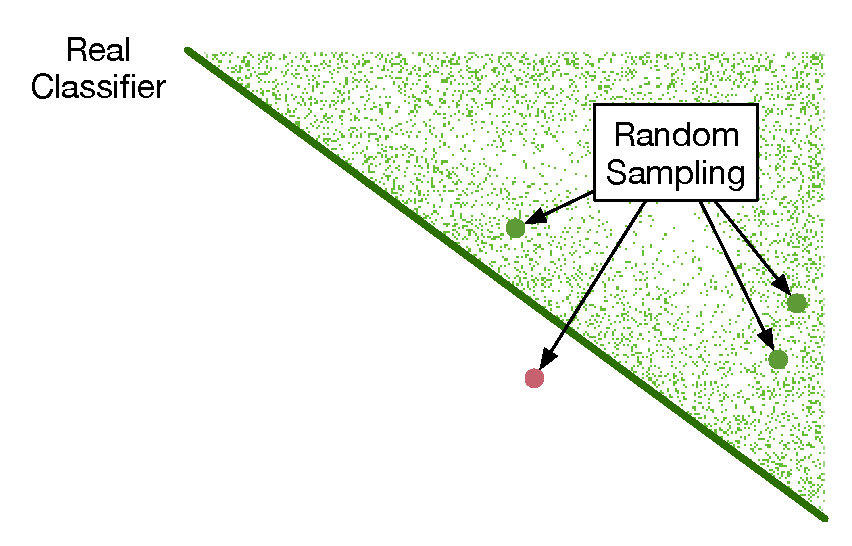
\includegraphics[scale=0.3]{figures/general-sampling-0.pdf}
%        \caption{Random Sampling}
        \centering
        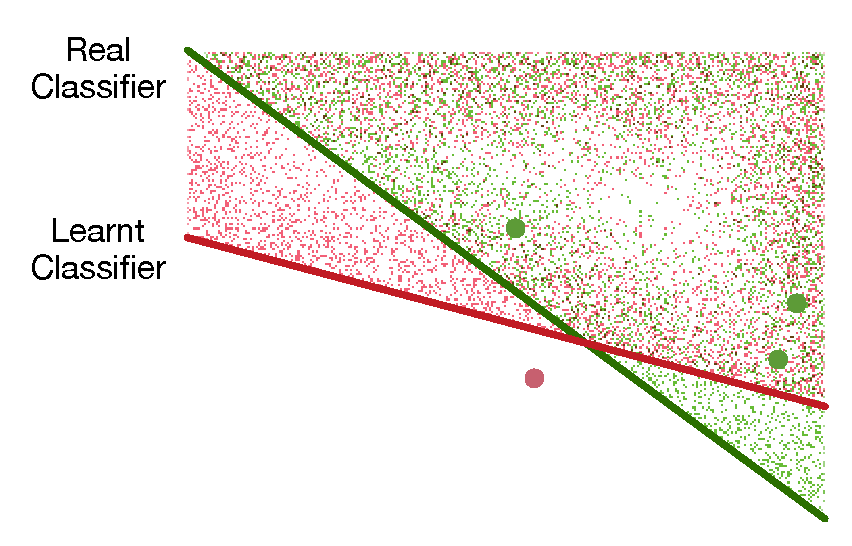
\includegraphics[scale=0.3]{figures/general-sampling-1.pdf} \\
%        \caption{Learnt Invariant}
        \centering
        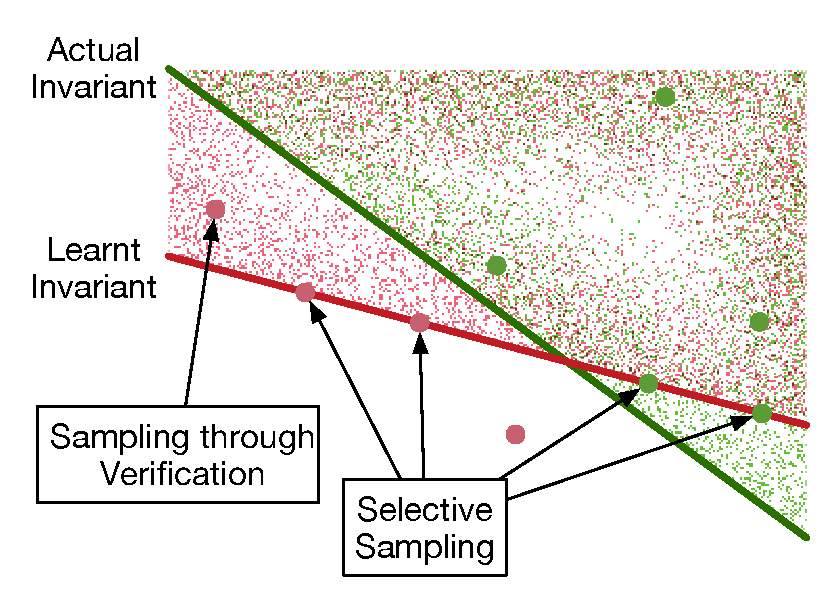
\includegraphics[scale=0.3]{figures/general-sampling-2.pdf}
%        \caption{Selective and Counter-Example Sampling}
        \centering
        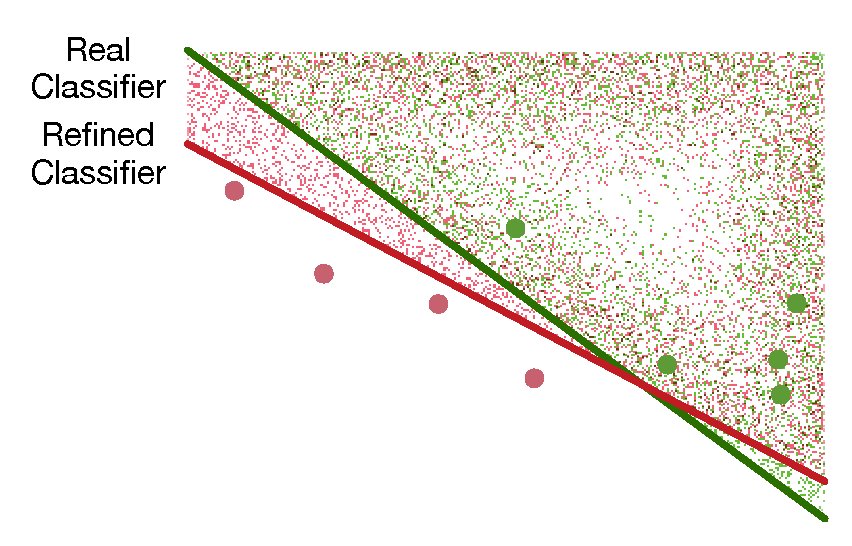
\includegraphics[scale=0.3]{figures/general-sampling-3.pdf}
%        \caption{Refined Invariant}
    \caption{Sampling approaches}
    \label{fig:sampling}
\end{figure}

\subsection{Making Use of Undetermined Samples} \label{alternative}
So far we have focused on learning and refining classifiers between $Positive(SP)$ and $Negative(SP)$ as candidate invariants. The question is then: how do we handle those valuations in $NP(SP)$? If we simply ignore them, there may be a gap between $Positive(SP)$ and $Negative(SP)$ and as a result, the learnt classifier may not converge to the invariant we want, even with the help of active learning.
This is illustrated in Figure~\ref{fig:running:example:sampling}, where the set of valuations in $Positive(SP)$ (marked with $+$), $Negative(SP)$ (marked with $-$) and $NP(SP)$ (marked with $?$) for the example in Figure~\ref{fig:running:example}(a) are visualized in a 2-D plane. Many samples between the line $x=y$ and $x-y=16$ may be contained in $NP(SP)$. As a result, without considering the samples in $NP(SP)$, a classifier located in the $NP(SP)$ region (e.g., $x - y \leq 10$, or $x - y \leq 13$) may be learned to perfectly classify $Positive(SP)$ and $Negative(SP)$. Worse, identifying more samples may not be helpful in improving the classifier if the new samples are in $NP(SP)$ (or can be classified correctly by the existing classifier).

 \begin{wrapfigure}{r}{5cm}
	 \vspace{-8mm}
\centering
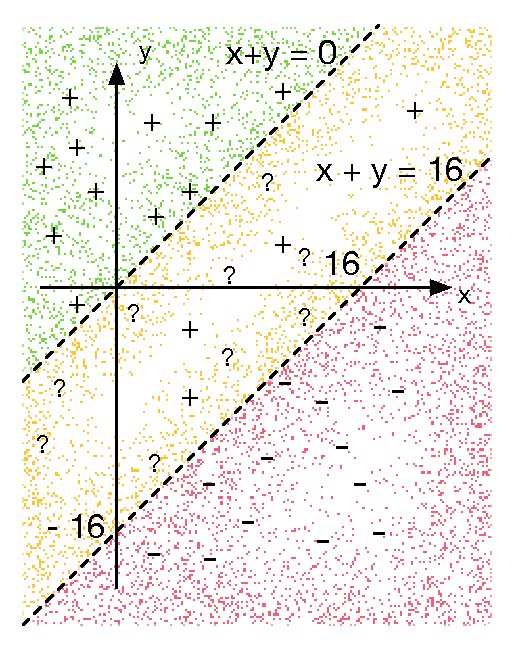
\includegraphics[scale=0.42]{figures/running-sampling.pdf}
 \caption{DTMC of \emph{egl} protocol.}
  \vspace{-6mm}
      \label{fig:running:example:sampling}
 \end{wrapfigure}

To overcome the problem, in addition to learn a classifier separating $Positive(SP)$ and $Negative(SP)$, we learn candidate invariants making use of $NP(SP)$. That is, we learn classifiers separating $Positive(SP)$ from $Negative(SP) \cup NP(SP)$ (i.e., assuming valuations in $NP(SP)$ fail the actual invariant), and classifiers separating $Negative(SP)$ from $Positive(SP) \cup NP(SP)$ (i.e., assuming valuations in $NP$ satisfy the actual invariant). For the example in Figure~\ref{fig:running:example}(a), if we focus classifiers in the form of linear inequalities, the classifier separating $Positive(SP)$ from the rest converges to $\textsc{null}$ (no such classifier), whereas the classifier separating $Negative(SP)$ from the rest converges to $x - y \leq 16$, which can be used to prove the Hoare triple. Note that we can apply different classification algorithms as well as active learning in learning these classifiers as well.

%\begin{figure}[t]
%      \centering
%      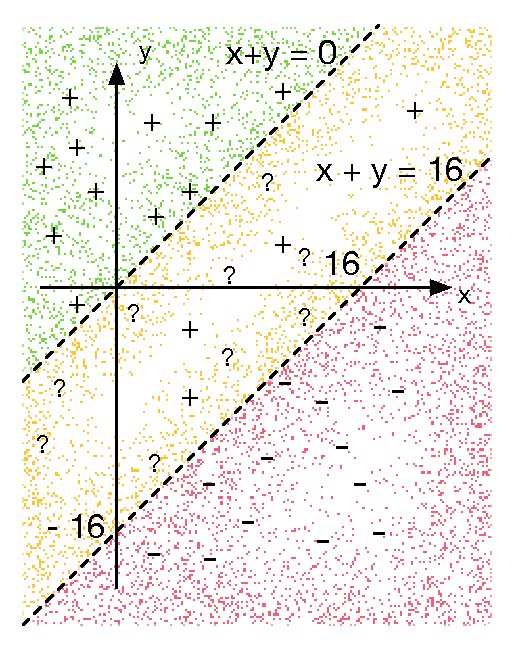
\includegraphics[scale=0.42]{figures/running-sampling.pdf}
%      \caption{Distribution of samples}
%      \label{fig:running:example:sampling}
%\end{figure}
%

%%!TEX root = paper.tex

\section{Active Learning} % (fold)
\label{sec:activelearning}
Active learning aims at generating candidate invariants through iterations of classification and selective sampling. Our overall algorithm for active learning is shown in Algorithm~\ref{alg:active}. The inputs of the algorithm include the set of samples $\mathit{SP}$; a classification algorithm $\mathit{classify}(P,N)$ which takes two sets of samples $P$ and $N$ and generates a classifier separating $P$ and $N$; and an algorithm for selective sampling $\mathit{selectiveSampling}$ which is often coupled with the classification algorithm. During each iteration of the loop from line 2 to 10, we apply $\mathit{classify}$ three times at line 3, 4 and 5 to learn three classifiers. The reason has been discussed in Section~\ref{sec:overview}. At line 6, we check whether any of the classifiers is different from the ones obtained during the last iteration. If none of them is, we return the three classifiers as candidate invariants at line 7, which will be verified afterwards. Otherwise, at line 9, we apply selective sampling to add more samples into $\mathit{SP}$ and then move on to the next iteration. We remark this algorithm is customizable in term of the classification algorithm and the corresponding selective sampling algorithm. In the following, we present two classification algorithms and selective sampling methods as examples.

\begin{algorithm}[t]
\SetAlgoVlined
\Indm
\Indp
Initialize $\mathit{old\_f_1}, \mathit{old\_f_2}, \mathit{old\_f_3}$ as $\textsc{null}$\;
\While{true} {
    $f_1$\ := \ $\mathit{classify}(\mathit{Positive}(\mathit{SP}), \mathit{Negative}(\mathit{SP}))$\;
    $f_2$\ := \ $\mathit{classify}(\mathit{Positive}(\mathit{SP}), \mathit{Negative}(\mathit{SP}) \cup \mathit{NP}(\mathit{SP}))$\;
    $f_3$\ := \ $\mathit{classify}(\mathit{Positive}(\mathit{SP}) \cup \mathit{NP}(\mathit{SP}), \mathit{Negative}(\mathit{SP}))$\;
    \If {for all $f_i$ where $i \in \{1,2,3\}$ such that $f_i = \mathit{old\_f_i}$} {
        \Return $f_1$, $f_2$, $f_3$\;
    }
    \For {$f_i$ where $i \in \{1,2,3\}$ such that $f_i \neq \textsc{null}$ and $f_i \neq \mathit{old\_f_i}$} {
        add $\mathit{selectiveSampling}(f_i)$ into $\mathit{SP}$\;
        $\mathit{old\_f_i}\ := \ f_i$\;
    }
}
\caption{Algorithm $\mathit{activeLearning}(\mathit{SP})$}
\label{alg:active}
\end{algorithm}
\vspace{-0.2cm}

% \subsection{Classification}
% In the machine learning community, many classification algorithms have been proposed, 
% e.g., perceptron~\cite{perceptron}, decision tree~\cite{quinlan1986induction}, $\mathit{SVM}$~\cite{svm:original} and neutral network~\cite{nn}.
% %Among plenty of classification approaches, \textsc{Zilu} takes Supported Vector Machines as a primary approach.
% %Before demonstrating the specific technique applied in \textsc{Zilu},
% %it should be noted that there are at least two main differences between machine learning problems and the problem in our setting:
% In our framework, the classification algorithms must generate perfect classifiers. 
% Formally, a perfect classifier $\phi$ for two sets of samples $P$ and $N$ is a predicate such that $s \models \phi$ for all $\mathit{s \in P}$ and $\mathit{s \not \models \phi}$ for all $\mathit{s \in N}$. 
% Furthermore, the classification algorithms must generate classifiers which are human-interpretable or can be handled by existing program verification techniques. 
% In the following, we present two such classification algorithms based on Support Vector Machine ($\mathit{SVM}$). 
% We remark that our framework is not restricted to $\mathit{SVM}$-based classification algorithms.
% %But there are still differences between the classification problem in machine learning field and the one in our framework:
% %\begin{itemize}
% %\item Our framwork need to learn an classifier with explicit form which is readable by human and can be proceeded by off-the-shelf constraints solvers.
% %However, the current machine learning techniques always produce an implicit classifier that is used to do prediction.
% %So we need to convert the implicit classifier to an explicit one, which will be used in later stage.
% %%Most machine learning techniques values more on prediction correctness rather than understanding the underlying problem. \LL{What is the difference?}
% %%although there is a research trend in machine learning to understand ongoing during these years.
% %%However, in the software engineering area, program verification cares about formalization and reasoning.
% %%Therefore, a classification technique from machine learning area would be highly suggested as long as it can predict correctly on newly received data.
% %%But in our setting, we need an explicit classifier which is readable by human and can be proceeded by off-the-shelf constraints solvers.
% %\item
% %%Machine learning algorithms consider more of generalization ability than classification correctness on the training data.
% %%Thus they would \LL{sacrifice the prediction correctness on the training data} for exchanging the higher generalization ability.  \LL{I feel our method is incorrect after reading this. Be precise. }
% %In our context, the classification accuracy on the training data is of vital importance,
% %and even a slight classification error can not be tolerated.
% %But some machine learning algorithms would partially sacrifice the classification correctness on the training data
% %for exchanging a higher prediction accuracy on the unseen data,
% %as they values the generalization ability most.
% %%On this basis, we hope the learned classifier can reflect the underlying logic of the given program.
% %% classification algorithm can have better generalization ability.
% %%\end{itemize}
% %Considering these differences,
% %in the following text,
% %we show our classification approaches which extend the native SVM to learning the invariant candidate.
% %\LL{I understand your meaning, but maybe say, we thus extend svm to capture ...
% %Do not describe methods in a vague manner. }


% %\subsection{Support Vector Machines}
% %\label{subsec:svm}
% %, is one of the most powerful approaches.
% %SVM is a supervised learning model with associated learning algorithms that analyze data used for classification.
% %In most setting, given a set of training examples, each marked as belonging to one of two categories,
% %an SVM training algorithm builds a model, which is a representation of the examples as points in space,
% %that can assign new examples into one category or the other,
% %making it a non-probabilistic binary linear classifier.
% $\mathit{SVM}$ is a supervised machine learning algorithm for classification and regression analysis~\cite{svm:original}. In this work, we use its binary classification functionality.
% In general, the binary classification functionality of (linear) $\textsc{Svm}$ works as follows.
% Given two sets of samples $P$ and $N$, $\mathit{SVM}$ generates a perfect linear classifier to separate them if there is any.
% In the following, we write $\mathit{svm}(P, N)$ to denote the function which returns a perfect linear classifier for $P$ and $N$ if there is any; or returns $\textsc{null}$ otherwise.
% We refer the readers to~\cite{svm:smo} for details on how the classifier is computed.
% In this work, we always choose the \textit{optimal margin classifier} (see the definition in~\cite{sharma2012interpolants}) if possible.
% Intuitively, the optimal margin classifier could be seen as the strongest witness why $P$ and $N$ are different.
% $\mathit{SVM}$ by default learns only classifiers in the form of a linear inequality (a.k.a.~a half space),
% e.g., in the form of $\mathit{a x + b y \geq c}$ where $x$ and $y$ are variables whereas $a$, $b$, and $c$ are constants.
% In practice, such classifiers may not be sufficient and thus, we develop algorithms to learn more expressive invariants.

% \paragraph{Polynomial Classifiers} Algorithm~\ref{alg:conjunctiveSVM} shows our algorithm for learning classifiers in the form of polynomial inequalities.
% The inputs of the algorithm include the two sets of samples $P$ and $N$ as well as a threshold on the maximum degree of the polynomial classifier.
% During the loop from line 2 to 7, we first map all the samples in $P$ (similarly $N$) to a set of samples $P'$ (similarly $N'$) in a high dimensional space using function $\mathit{mapToDegree}$.
% Given a set of samples $X$ and a target degree, function $\mathit{mapToDegree}$ returns a set of new samples $X'$ such that each element in $X$ is mapped to an element in $X'$.
% For instance, let $\{x \mapsto 2, y \mapsto 1\}$ be an element in $X$ and the target $\mathit{degree}$ be 2, the following element is added to $X'$: $\{x \mapsto 2, y \mapsto 1, x^2 \mapsto 4, xy \mapsto 2, y^2 \mapsto 1\}$.
% That is, given a valuation in $P$, we systematically add all terms constituted by the same variables with a degree no more than $\mathit{degree}$, as if they are new variables.
% %The primary idea is simple, after mapping raw data (program states) from original space in $\mathcal{S}^+$, $\mathcal{S}^-$ and $\mathcal{S}^\rightarrow$ to a high dimensions,
% $\mathit{SVM}$ is then applied to learn a perfect linear classifier for $P'$ and $N'$. % as is shown in~\ref{subsec:svm}.
% Mathematically, a linear classifier in the high dimensional space is the same as a polynomial classifier in the original space~\cite{svm:kernel}.
% In order to favor classifiers with lower degrees (which often are easier to understand or verify), we start with looking for a polynomial classifier with degree 1 and only look for higher-degree polynomial classifiers if we find no lower-degree ones.
% The algorithm terminates when we reach the threshold on the maximum degree.
% We remark that the size of each sample in $P'$ or $N'$ grows rapidly with $\mathit{degree}$. 
% %The number of monomials of $\mathit{degree}$ in $\mathit{n}$ is $(^{n+degree-1}_{degree})$.
% However, in our experiments, we can often identify useful classifiers with a small value for $\mathit{degree}$.
% We remark that the polynomial classifiers learnt by Algorithm~\ref{alg:polynomialSVM} can represent classifiers in the form of disjunctive or conjunctive linear inequalities.
% %Because some invariants of conjunctive or disjunctive form can be expressed in polynomials equivalently,
% For instance, the classifier $\big((x \ge d_0) \wedge (x \le d_1)\big) \vee (x \ge d_2)$
% where $\mathit{d_0 < d_1 < d_2}$ are constants can be represented as: $\mathit{x^3 + (d_0d_1 + d_0d_2 + d_1d_2)x^2 - (d_0 + d_1 + d_2)x - d_0d_1d_2 \geq 0}$.

% \begin{algorithm}[t]
% \SetAlgoVlined
% \Indm
% \Indp
%     Initialize $degree$ as 1\;
%     \While {$degree \le \mathit{max\_degree}$} {
%         $P' := \mathit{mapToDegree}(P, \mathit{degree})$\;
%         $N' := \mathit{mapToDegree}(N, \mathit{degree})$\;
%         \If {$\mathit{svm}(P', N')$ is not $\textsc{null}$} {
%             \Return $\mathit{svm}(P', N')$\;
%         }
%     	$\mathit{degree} := \mathit{degree} + 1$\;
%     }
%     \Return $\textsc{null}$;
% \caption{Algorithm $\mathit{polynomial}(P,N)$}
% \label{alg:polynomialSVM}
% \end{algorithm}
% \vspace{-2mm}
% \begin{algorithm}[t]
% \SetAlgoVlined
% \Indm
% \Indp
%     Initialize set $C$\ as an empty set $\{\}$, set $\mathit{Misclassified}$\ as\ $N$\;
%     \While {$\mathit{Misclassified}$ is not empty} {
%         Random choose $s$ from $\mathit{Misclassified}$\;
%         $f := \mathit{polynomial}(P, \{s\})$\;
%         Add $f$ into $C$\;
%         \For {$s' \in \mathit{Misclassified}$} {\
%             \If {$f(s') < 0$} {
%                 remove $s'$ from $\mathit{Misclassified}$\;
%             }
%         }
%     }
%     Minimize $C$\;
%     \Return the conjunction of all predicates in $C$;
% \caption{Algorithm $\mathit{conjunctivePoly}(P, N)$}
% \label{alg:conjunctiveSVM}
% \end{algorithm}

% %The whole classification algorithm is described in Algorithm~\ref{alg:classify}.
% %Note that,
% %$\textsc{Svm}$ in this algorithm can be substitute with other classification techniques for different learning purposes.
% %We will take two classification algorithms as examples to demonstrate this promotion in \LL{?}~\ref{subsec:svm:derivatives}.
% %\begin{algorithm}[!h]
% %\SetAlgoVlined
% %\Indm
% %\KwIn{$\mathcal{S}^+$, $\mathcal{S}^-$, and $\mathcal{S}^\rightarrow$}
% %\KwOut{$\textsc{Null}$ or a perfect classifier for $\mathcal{S}^+$ and $\mathcal{S}^-$ without violating $\mathcal{S}^\rightarrow$}
% %\Indp
% %    let $f$ = $\textsc{Svm}$($\mathcal{S}^+$, $\mathcal{S}^-)$\;
% %    \If {$f$ violates any data in $\mathcal{S}^+$ or $\mathcal{S}^-$} {
% %        \Return $\textsc{Null}$\;
% %    }
% %    \If {$f$ violates any inference rules in $\mathcal{S}^\rightarrow$} {
% %        \Return $\textsc{Null}$\;
% %    }
% %    \Return $f$;
% %\caption{Algorithm $classify$}
% %\label{alg:classify}
% %\end{algorithm}



% %In the following, we present how we obtain a classifier automatically using $\textsc{Svm}$.
% %In this work, we always choose the \textit{optimal margin classifier} (see the definition in~\cite{Sharma2012}) if possible.
% %This half space could be seen as the strongest witness why the two data states are different.
% %In the following, we write $svm(S^+, S^-)$ to denote the function which returns a linear classifier

% %\subsection{Checking}
% %With the learned $\textsc{Svm}$ model,we check whether it can perfectly classify these states first.
% %If yes, then we can automatically turn it back to a hyperplane form, which is regarded as our invariant candidate.
% %Otherwise, we may apply other classification techniques for learning, which will be mentioned at ``$\textsc{Svm}$ derivatives'' part in the end of this section.


% %\subsection{SVM Derivatives}
% %\label{subsec:svm:derivatives}
% %%$\mathcal{S}^+$, $\mathcal{S}^-$, and $\mathcal{S}^\rightarrow$
% %If $\mathcal{S}^+$, $\mathcal{S}^-$ cannot be classified with 100\% accuary by one half-space only,
% %a more complicated function $f$ must be adopted.
% %For instance, there has been research on invariants in form of conjunctives~\cite{sharma2012interpolants},
% %octagonal~\cite{mine2006octagon}, tree form~\cite{krishna2015learning}\cite{garg2015learning} and so on.
% %
% %%For instance, if there is a classifier in the form of conjunctive of multiple half spaces,
% %%the algorithm presented in~\cite{sharma2012interpolants} can be used to identify such a classifier.
% %
% %Moreover, as is noted Algorithm~\ref{alg:classify} can be easily extended by substituting $\textsc{Svm}$ with other classification approaches,
% %\textsc{Zilu} has implemented two classification algorithms by extending the native $\textsc{Svm}$:
% %$Polynomial \textsc{Svm}$ for learning invariants in the form of polynomials or any equivalent expressions,
% %and $Conjunctive$\textsc{Svm} for learning invariants in the form of conjunctives.
% %
% %\medskip\noindent
% %\textbf{Polynomial SVM.}
% %In previous research, several papers ~\cite{**} have studied invariants with conjunctive form or disjunctive form.
% %However, there is still no efficient approach to learning these invariants.
% %In our research, we found sometimes convert the conjunctive or disjunctives to a polynomial expression might be a nice try to this problem.
% %In the real work, there are not only linear invariants but invariants of many other forms,
% %such as, conjunctives~\cite{sharma2012interpolants}, octagonal~\cite{mine2006octagon}, polynomial, and tree form~\cite{krishna2015learning}\cite{garg2015learning}.
% %In this part, we present our classification approach based on primitive \textsc{Svm} for learning polynomial invariants,
% %which have not been discussed by previous research.
% %In this part, we would like to learn this kind of invariants.
% %Apparently methods that use linear template or linear classification algorithm do not work.
% %Actually, polynomials are more powerful on this than they look at the first glance, especially univariate polynomials.
% %Some cubic univariate polynomials can represent disjunctive of a conjunctive expression and a linear expression.
% %For example, the following two expressions are equivalent:
% %$$\big(x \ge x_0 \bigwedge x \le x_1) \bigvee x \ge x_2\big) \ where\ x_0 < x_1 < x_2$$
% %$$x^3 + (x_0x_1 + x_0x_2 + x_1x_2)x^2 - (x_0 + x_1 + x_2)x - x_0x_1x_2 >= 0$$
% %This leads us to develop a classification algorithm for learning polynomial divider.
% %
% %The whole procedure is shown in algorithm~\ref{alg:polynomialSVM}.
% %In practice, \textsc{Zilu} provide polynomials up to degree 4 as we think degree 4 can cover most hackneyed invariants for now.


% %\begin{align}
% %    x^3 + a\dot x^2 - b\dot x - c &>= &0 \\
% %    where a &= & x_0 \dot x_1 + x_0 \dot x_2 + x_1 \dot x_2 \\
% %\end{align}
% %For instance, if the target invariant is
% %$$(x \ge x_0) \vee (x \le x_1) \ where\ x_0 < x_1$$
% %we can find an equivalent polynomial expression:
% %$$x^2 - (x_0 + x_1)x + x_0x_1 \ge 0$$
% %So $polynomialSVM$ can be used to learn a polynomial classifier or any complex expression as long as it can be expressed in form of polynomials.

% \paragraph{Conjunctive Polynomial Classifiers}
% As discussed above, polynomial classifiers can equivalently represent certain conjunction or disjunction of linear classifiers. It is however not always possible, i.e., some conjunctive or disjunctive linear inequalities cannot be expressed in the form of a polynomial classifier. A simple example is $\mathit{x \ge 0 \land y \ge 0}$. Thus, we develop an algorithm to learn more expressive classifiers.

% Algorithm~\ref{alg:conjunctiveSVM} shows a classification algorithm which is designed to learn conjunctive polynomial classifiers.
% %So in this part, we introduce the algorithm to learn conjunctive invariants directly.
% %, avoiding the tries to convert them into a form of polynomials.
% It is inspired by the algorithm presented in~\cite{sharma2012interpolants}. The difference is that~\cite{sharma2012interpolants} learns conjunctive linear classifiers, whereas we learn conjunctive polynomial classifiers. The idea is to pick one sample $s$ from $N$ (at line 3) each time and identify a polynomial classifier based on Algorithm~\ref{alg:polynomialSVM} separating $P$ and $\{s\}$ (a.k.a.~a clause). Next, we remove (at line 6 to 8) all samples from $N$ which can be correctly classified by the polynomial classifier found at line 4, and then repeat the process until $N$ becomes empty.
% %Compared to the classification algorithm presented in~\cite{sharma2012interpolants}, Algorithm~\ref{alg:conjunctiveSVM} learns conjunctive polynomial classifiers whereas the one in~\cite{sharma2012interpolants} is limited to conjunctive linear classifier. The more important difference is however our classification algorithm is coupled with a selective sampling procedure.
% At line 10, we minimize $C$ by identifying and removing any $f$ in $C$ such that the conjunction of the remaining predicates in $C$ perfectly classifies $P$ and $N$ still. We remark that Algorithm~\ref{alg:conjunctiveSVM}, like the one in~\cite{sharma2012interpolants}, may learn a classifier with many clauses, as one clause is introduced each time line 5 is executed. In the worse case, if each polynomial classifier found at line 4 only classifies the one sample $s$, the returned $C$ would conjunct as many clauses as the number of samples in $N$. Selective sampling, as we discuss below, helps to tame this problem, if there exists a conjunctive polynomial classifier with fewer clauses.





%\section{Active Learning}
%Due to the limited set of samples we have (which is often referred to as labeled samples in the machine learning community),
%the guessed classifier obtained from the previous iteration might be far from being correct.
%In fact, without labeled samples which are right on the boundary of the `actual' classifier,
%it is very unlikely that we would find it.
%Intuitively, in order to get the `actual' classifier, we would require samples which would distinguish the actual one from any nearby one.
%This problem has been discussed and addressed in the machine learning community using active learning and selective sampling~\cite{DBLP:conf/icml/SchohnC00}.

%The concept of active learning or selective sampling refers to the approaches
%that aim at reducing the labeling effort by selecting only the most informative samples to be labeled.
%SVM selective sampling techniques have been proven effective in achieving a high accuracy
%with fewer examples in many applications~\cite{DBLP:conf/mm/TongC01,DBLP:journals/jmlr/TongK01}.
%The basic idea of selective sampling is that at each round,
%we select the samples that are the closest to the classification boundary so that they are the most difficult to classify and the most informative to be labeled.
%Since an SVM classification function is represented by support vectors which are the samples closest to the boundary,
%this selective sampling effectively learns an accurate function with fewer labeled data~\cite{DBLP:conf/icml/SchohnC00}.
%In our setting, this means that we should sample a program state right by the classifier and test the program
%with that state to label that feature vector so that the classifier would be improved.


% section classification (end)

\paragraph{Selective Sampling} \label{subsec:active:learning}
Selective sampling is helpful in reducing the number of required samples. 
Often, different selective sampling methods are adopted according to different classification algorithms. 
In the following, we show how selective sampling works for the two above-mentioned classification algorithms. %We refer the readers to~\cite{???} on a survey on how selective sampling works in general.

Assume that we adopt Algorithm~\ref{alg:polynomialSVM} in our framework and learn a polynomial classifier: $\mathit{-4x^2+2y \geq -11}$. 
Following the idea in~\cite{DBLP:conf/icml/OrabonaC11}, the following procedure is applied to identify samples right on the classification boundary for improving the classifier.
\begin{enumerate}
\item Choose a variable in the classifier, for example, $x$.
\item Generates random value for other variables. For example, we let $y$ be $12$.
\item Solve the equation $\mathit{-4x^2+2y = -11}$ after substituting variables with their values. If there is no solution, go back to (1) and retry. 
In our example, $\mathit{x \approx 2.9580}$.
%\item Add a random variance $\epsilon \in [-1, 1]$ to the value of the picked variable. Here we add $\epsilon = 0.4$ to the value of $x$, and thus the new value of $x$ is $3.3580$.
\item Roundoff the values of all the variables according to their types in the given program. In our example, we obtain the valuation $\mathit{\{x \mapsto 3, y \mapsto 12\}}$.
\end{enumerate}
Alternatively, we can use existing equation system solvers directly to find solutions for equation $\mathit{-4x^2+2y = -11}$. 
If Algorithm~\ref{alg:conjunctiveSVM} is adopted to learn conjunctive polynomial classifiers, we apply the above procedure to each and every polynomial clause in the classifier to obtain new samples. 
While it is easy to see that the classifiers learnt in Algorithm~\ref{alg:active} may improve through the iterations (since more samples are available), 
it is hard to predict how fast it converges. 
We evaluate the effectiveness of these classification algorithms as well as selective sampling methods empirically in the next section.
%Having a classifier for the current dataset ($\mathcal{S}^+$, $\mathcal{S}^-$, and $\mathcal{S}^\rightarrow$),
%active learning technique keeps refining the classifier until it gets converged.
%That means the classifier remains identical even adding more data points into the training set.
%Algorithm~\ref{alg:active} presents details on how active learning is implemented in \textsc{Zilu}.
%
%
%
%At line 3, we obtain a classifier based on Algorithm~\ref{alg:classify}.
%We compare the newly obtained classifier with the previous one at line 4, if they are identical, we return the classifier;
%otherwise, we apply selective sampling so that we can generate additional labeled samples for refining the classifier.
%%\LL{should be used to check the correctness?}
%In particular, at line 9, we apply selective sampling~\cite{DBLP:conf/icml/SchohnC00} to generate most informative samples.
%Notice that in our setting, as indicated in Section ~\ref{sec:sampling}, the most informative samples are those which are exactly on the lines
%and therefore can be obtained by solving an equation system using libraries.
%At line 10 and line 11, we test the program with the newly generated samples so as to label them accordingly.

%\begin{example}
%\LL{to be added}
%\end{example}

%\begin{proposition}
%Algorithm $activeLearning$ always eventually terminates. \hfill \qed
%\end{proposition}


\vspace{-0.3cm}
%!TEX root = paper.tex

\section{Evaluations} % (fold)
\label{sec:evaluations}
We have implemented our invariant inference framework in a tool, called \textsc{Zilu}. \textsc{Zilu} is written using a combination of C++ as well as shell codes (for invoking external tools).
\textsc{Zilu} makes use of GSL~\cite{gough2009gnu} to solve equation systems which is necessary for selective sampling and
%% uses
 LibSVM~\cite{chang2011libsvm} as a primitive classification engine for
SVM-based learning classifier. %% based on SVM.
For invariant verification, we %% reuse a large part of
adopt the KLEE project~\cite{cadar2008klee} to
symbolically execute
%% generate verification conditions for
 C programs %% and use
prior to invoke Z3~\cite{de2008z3} for checking satisfiability of
the formulas (4), (5) and (6).
 We remark that KLEE is a concolic symbolic executor; it may
concretely execute the programs and return 
 under-approximated
abstraction. This may affect the soundness of our system.
To overcome this problem, we detect those path conditions produced from
concrete executions
and return sound abstraction, i.e. $true$, for them.
 %% KLEE was designed for test case generation and thus its default encoding may result in under-approximation of the program behavior. We have re-implemented the relevant part of KLEE to make sure the right verification conditions are generated.

Our test subjects include a set of benchmark programs %% which we
(i) gathered from
 the previous publications on loop invariant generation~\cite{???}  as well as
 (ii)
%% benchmark programs
taken  from
 the software verification competition repository~\cite{Dirk:SVCOMP:2016}.
All benchmarks are available from~\cite{zilu}.
%% Note
We notice that loops of these benchmark programs often contain non-deterministic choices
%% in the loop
which are used to model I/O environment (e.g., an external function call).
As non-determinism is beyond the scope of this paper,
we syntactically replace these non-deterministic commands by  free boolean-type variables.
It would be interesting to investigate how
 our active learning verification system can be extended
to infer non-determinism-based invariants.
 %% which by our assumption is not allowed. We thus transform the programs so that free boolean-type variables are introduced to replace the non-deterministic choice. We remark that the assumption of no non-determinism is less a problem for verification programs in practice as they are often deterministic. These benchmark programs are made non-deterministic often as a way of abstracting away certain complicated (e.g., an external function call) part of the program which is irrelevant to proving/disproving the Hoare triple.
%In our experimental evaluation,
%we test \textsc{Zilu} with \LL{Number} loop invariant benchmarks
%in the following form, where $\mathit{Body}$ can have nested loops and conditional choices.
%\[
%   \{ \mathit{Pre} \} \mathit{while}(\mathit{Cond}) \{ \mathit{Body} \} \{ \mathit{Post} \}
%\]
%% Do not apply this to `add' more content to the paper.
%% It lefts lots of empty space which did the contrary thing.
%% \begin{align*}
%% &Pre&\\
%% &while (Cond) \{&\\
%% &  \quad Body &\\
%% &\} &\\
%% &Post &
%% \end{align*}
%\LL{Introduce the sources of the benchmark.}
 %% All benchmarks are available from~\cite{zilu}.

The parameters chosen in our experimental evaluation are as follows.
For random sampling, we generate random values of all input variables of the program from their default ranges. Be default, we generate XXX random samples. 
%which would be enlarged if we can not find samples in a few tries.
%Our experiments indicate this $\mathcal{R}$ is a relatively rational range for the initial sampling.
During classification, the parameter $C$ which is the preference between avoiding misclassifying each training example and enlarging decision boundary,
and the inner iteration for SVM learning are set to their maximum value so as to generate only perfect classifiers. Each invocation of the SVM classification engine is set to time out in XXX seconds. The maximum dimension for learning polynomial classifiers is set to be 3. For invariant verification, we encode integer-type variables in the programs as integers in Z3. 


%Considering the differences between machine learning problem and our setting,
%\textsc{Zilu} tunes $\textsc{LibSvm}$~\cite{chang2011libsvm} in the following three aspects in order to get a \underline{perfect classifier}.
%\begin{itemize}
%\item Convert \textsc{Svm} model to an explicit classifier.
%The original \textsc{Svm} technique does not explicitly calculate a hyperplane, but emits its own model
%which can be used to do prediction on the given data.
%%This might not a big problem if we do not apply $\textsc{Svm}$ with some kernel method (which is used to classify no linear separable data).
%However, we need a explicit classifier as the loop invariant candidate which can be understood and proceeded later for verification.
%(This is also why we do not apply $\textsc{Svm}$ with kernel methods~\cite{yu2009evolving},
%considering converting $\textsc{Svm}$ models with kernel methods, i.e. $\textsc{Rbf}$ kernel, would be a complicated, sometimes even impossible, task.)
%
%\item As \textsc{Zilu} treasures classification accuracy on the training dataset% than anything else,
%before applying primitive $\textsc{Svm}$ technique, the parameters
%(mainly $C$ which tells the $\textsc{Svm}$ optimization how much you want to avoid misclassifying each training example)
%%different from $\mathcal{C}$ used as loop invariant candidate in our context)
%should be carefully tuned to learn a perfect classifier which perform well on the training points.
%
%\item Validating the learned classifier.
%Checking the classification correctness of the learned classifier
%on $\mathcal{S}^+$ and $\mathcal{S}^-$ is still needed as our setting needs to ensure the learned classifier is a perfect one.
%\textsc{Zilu} also takes $\mathcal{S}^\rightarrow$ to validate the learned classifier(as is shown in Section~\ref{sec:sampling}).
%\end{itemize}

\begin{table}[t]
\scriptsize
\centering
\caption{Statistics on TLV abstracting the classes, where N.A. stands for not available}
%\begin{tabular}{l c | c c c c | c c c c | c c }
%\cline{3-10}
\begin{tabular}{l c | c c c c| c c c | c c }
\cline{3-9}
%& &\multicolumn{4}{|c|}{\textsc{Zilu} with Selective}&\multicolumn{4}{c|}{\textsc{Zilu} without Selective} & & \\
& &\multicolumn{4}{|c|}{\textsc{Zilu} with Selective}&\multicolumn{3}{c|}{\textsc{Zilu} without Selective} & & \\
\hline
%\multicolumn{1}{|c|}{benchmark}&\multicolumn{1}{|c|}{inv type}& $\sharp$r. sample & $\sharp$s. sample & $\sharp$v. sample & time & $\sharp$r. sample & & $\sharp$v. sample & time & \multicolumn{1}{|c|}{Interproc} & \multicolumn{1}{|c|}{CPAChecker} \\
\multicolumn{1}{|c|}{benchmark}&\multicolumn{1}{|c|}{inv type}& $\sharp$r. samples & $\sharp$s. samples & $\sharp$v. samples &time(s) & $\sharp$r. samples & $\sharp$v. samples &time(s) & \multicolumn{1}{|c|}{Interproc} & \multicolumn{1}{|c|}{CPAChecker} \\
\hline % inserts single horizontal line
\multicolumn{1}{|c|}{afnp2014\_true\text{-}unreach\text{-}call}         	&conjunctive	&1056 &4224 & &259.38	&5160 & &295.03  & &  \\
\multicolumn{1}{|c|}{cav12foo1}         									&conjunctive 	&228 &912 &20 &51.07	&1980 &48 &168.97  & &  \\
\multicolumn{1}{|c|}{cav12foo2}         									&conjunctive 	&36 &144 &2 &16.09		&260 &6 &15.98  & &  \\
\multicolumn{1}{|c|}{cggmp2005\_variant\_true\text{-}unreach\text{-}call}   &conjunctive 	&210 &840 & &74045	&2220 & &timeout  & &  \\
\multicolumn{1}{|c|}{conj}         											&polynomial 	&10 &40 &2 &20.48		&70 &1 &28.48  & &  \\
%\multicolumn{1}{|c|}{conj}         											&conjunctive/polynomial & & &  &   &  & & &  & &  \\
\multicolumn{1}{|c|}{css2003\_true\text{-}unreach\text{-}call}         		&conjunctive 	&140 &560 & &36.02	&1220 & &83.29  & &  \\
\multicolumn{1}{|c|}{dis}         											&polynomial 	& & & &  &   & &  & &  \\
\multicolumn{1}{|c|}{down\_true\text{-}unreach\text{-}call\_1}         		&conjunctive 	&114 &256 & &116.21  &2160  &  &timeout  & &  \\
\multicolumn{1}{|c|}{down\_true\text{-}unreach\text{-}call\_2}         		&conjunctive 	&132 &528 & &27.5  &360 &   &timeout  & &  \\
\multicolumn{1}{|c|}{f2}         											&linear 		&52 &208 &1 &10.15  &120 &1   &12.03  & &  \\
\multicolumn{1}{|c|}{f3}         											&linear 		&36 &144 &1 &105.15  &330  &5  &93.04  & &  \\
%\multicolumn{1}{|c|}{fig1a\_1}         										&linear & & &  &   &  & & &  & &  \\
%\multicolumn{1}{|c|}{fig1a\_2}         										&linear & & &  &   &  & & &  & &  \\
\multicolumn{1}{|c|}{interproc\_test1}         								&linear 		&8 &32 &1 &9.21  &40 &2   &10.38  & &  \\
\multicolumn{1}{|c|}{interproc\_test2}         								&linear 		&84 &96 &1 &11.66  &240  &1  &171.14  & &  \\
\multicolumn{1}{|c|}{interproc\_test3}         								&linear 		&42 &168 &1 &30.32  &420 &5   &43.34  & &  \\
\multicolumn{1}{|c|}{interproc\_test4}         								&linear 		&28 &112 &4 &14.8  &240 &5   &38.25  & &  \\
\multicolumn{1}{|c|}{interproc\_test5}         								&linear 		&32 &128 &1 &9.18  &180 &3   &28.05  & &  \\
\multicolumn{1}{|c|}{interproc\_test6}         								&polynomial 	&6 &24 &1 &11.83  &70  &2  &18.27  & &  \\
\multicolumn{1}{|c|}{interproc\_test8}         								&conjunctive 	&24 &96 &6 &22.13  &220  &2  &97.47  & &  \\
\multicolumn{1}{|c|}{interproc\_test11}         							&linear 		&24 &96 &2 &24.79  &180 &2   &206.07  & &  \\
\multicolumn{1}{|c|}{lili2}         										&linear 		&84 &336 &4 &21.28  &720  &9  &82.24  & &  \\
\multicolumn{1}{|c|}{linear6}         										&linear 		&18 &72 &1 &16.19  &270 &3  &179.39  & &  \\
\multicolumn{1}{|c|}{multivar\_true\text{-}unreach\text{-}call1}         	&conjunctive 	&68 &272 &3 &16.84  &220 &4   &15.22  & &  \\
\multicolumn{1}{|c|}{terminator\_01\_safe}         							&linear 		&6 &24 &1 &9.2  &90  &4  &13.06  & &  \\
\multicolumn{1}{|c|}{test}         											&linear 		&28 &112 &1 &10.19  &420 &2  &24.51  & &  \\
\multicolumn{1}{|c|}{test2}         										&conjunctive 	&44 &176 &3 &79.45  &120  &3  &timeout  & &  \\
%\multicolumn{1}{|c|}{up\_true\text{-}unreach\text{-}call\_1}         		&conjunctive & & &  &   &  & & &  & &  \\
\multicolumn{1}{|c|}{up\_true\text{-}unreach\text{-}call\_2}         		&conjunctive 	&240 &960 &14 &84.02  &540 &7   &89.77  & &  \\
%\multicolumn{1}{|c|}{xeq10}         										&linear & & &  &   &  & & &  & &  \\
\multicolumn{1}{|c|}{xle10}         										&linear 		&6 &24 &1 &8.57  &60 &3   &12.58  & &  \\
\multicolumn{1}{|c|}{xy10}         											&linear 		&162 &648 &4 &39.69  &840  &11  &40.51  & &  \\
\multicolumn{1}{|c|}{xyle0}         										&polynomial 	& & & &  &   & &  & &  \\
\hline
\end{tabular}
\label{tbl:stats}
\end{table}

%\begin{table*}[t]
%    \begin{center}
%    % \begin{minipage}{\textwidth}
%    % \begin{adjustwidth}{-1in}{-1in}
%    \begin{center}
%    \begin{adjustbox}{max width=1\textwidth}
%    \begin{tabular}{l | r | r | r | r | r | r | r | r | r}
%        \hline\hline
%        Benchmark
%            & $\sharp$Random Samples & $\sharp$Selective Samples & $\sharp$Iterations
%            & $\sharp$Traces & $\sharp$Variables
%            & Time & Invariant Type
%            & Interproc & CPAChecker
%            \\
%        \hline
%        Linear 1
%            & 196 & 4 & 1
%            & 1 & 1
%            & 3.31s & Linear
%            & 0.01s & 3.42s
%            \\
%        \hline
%        Linear 2
%            & 3158 & 7 & 1
%            & 1 & 2
%            & 9.86s & Linear
%            & 0.01s & 3.29s
%            \\
%        \hline
%        Linear 3
%            & 11102 & 6 & 1
%            & 1 & 3
%            & 40.24s & Linear
%            & 0.01s & 3.50s
%            \\
%        \hline
%        Linear 4
%            & 1143 & 10 & 1
%            & 9 & 2
%            & 12.54s & Linear
%            & 0.01s & 3.76s
%            \\
%        \hline
%        Linear 5
%            & 918 & 8 & 2
%            & 3 & 2
%            & 14.47s & Linear
%            & Error & 3.66s
%            \\
%        \hline
%        Poly 1
%            & 64 & 7 & 2
%            & 1 & 1
%            & 10.51s & Polynomial
%            & Unknown & Unknown
%            \\
%        \hline
%        Poly 2
%            & 32711 & 85 & 7
%            & 2 & 2
%            & 23m43.1s & Polynomial
%            & Unknown & Unknown
%            \\
%        \hline
%        Poly 3
%            & 272 & 17 & 4
%            & 3 & 1
%            & 15.82s & Polynomial
%            & 0.01s & 3.31s
%            \\
%        \hline
%        Poly 4
%            & 2287 & 112 & 9
%            & 2 & 2
%            & 13m43.7s & Polynomial
%            & Unknown & Unknown
%            \\
%        \hline
%        Conjunction 1
%            & 21247 & 81 & 1
%            & 3 & 2
%            & 20m41.35s & Conjunction
%            & 0.01s & 3.16s
%            \\
%        \hline
%    \end{tabular}
%    \end{adjustbox}
%    \end{center}
%    % \end{adjustwidth}
%    % \end{minipage}
%    \end{center}
%    \caption{Experiment Results}
%    \label{tab:experiments}
%\end{table*}

We compared \textsc{Zilu} with two state-of-the-art invariant inference tools: Interproc~\cite{jeannet2010interproc} and CPAChecker~\cite{beyer2011cpachecker}. We remark many other tools have been reported~\cite{}, most of which are not maintained any more. The comparison between \textsc{Zilu} and Interproc or CPAChecker should be taken with a grain of salt as the methods for invariant generation are very different. Interproc is based on abstract interpretation. In the experiment, Interproc uses its most expressive abstract domain, i.e., the reduced product of polyhedra and linear congruences abstraction. Similar to \textsc{Zilu}, Interproc explicitly labels the loop invariants in the loop program. We thus can manually check their correctness and compare them with the invariants generated by \textsc{Zilu}. On the other hand, CPAChecker (formerly BLAST~\cite{henzinger2003software}) is a software verification tool based on the framework of configurable program analysis~\cite{beyer2007configurable}. In the experiment, CPAChecker is configured to generate loop invariants to prove the same Hoare triple. In addition, we compare the performance of \textsc{Zilu} with or without active learning in order to show the relevance of active learning and selective sampling.

The experiment results are presented in Table~\ref{tbl:stats}. All of the experiments are conducted using x86\_64 Ubuntu 14.04 (kernel 3.13.0-85-generic) with 2.3 GHz Intel Core i5 and 4G 1333MHz DDR3.
The first column shows which a name of the benchmark program. The second shows the type of invariant required for proving the Hoare triple. The next four columns present details on \textsc{Zilu}, i.e., the number random samples, selective samples, samples through verification and the execution time. The next four present the corresponding statistics running \textsc{Zilu} without selective sampling. The last two columns show the execution time of the two comparing tools.  
%%\LL{I need more information on the percentage of the samples. }
%`$\sharp$Invariants' stands the numbers of invariants generated by SVM,
%and `$\sharp$Iterations' represents the number of invariant candidates.
%Notice that an invariant generated by SVM becomes an invariant candidate
%when it converges to two previously generated invariants from SVM in one iteration process.
%`$\sharp$Traces' represents the number of loop body traces produced by KLEE~\cite{cadar2008klee}.
%and `$\sharp$Variables' represents the number of program variables.
% In general, when numbers of traces and variables increase in a program,
% the invariant inference difficulty increases.
%The seventh column gives the time used for the invariant generation
%and the eighth column gives the invariant type of the generated invariant.
We remark that since \textsc{Zilu} relies on generating random numbers, all numbers collected from \textsc{Zilu} in the table are the average of 10 experiments.

As can be seen from Table~\ref{tab:experiments},
some of the experiments take much longer time comparing with others,
with high numbers of samples, invariants, iterations.
The reason behind this is
that some variables are missing in the constraints of the loop invariant,
e.g., `Poly 2', `Poly 4' and `Conjunction 1'.
For instance, in the `Poly 1' case, the loop invariant is `$x^2 \le y^2$'.
However, the general form of a 2-order polynomial with 2 variables
is written as
\[
    a \cdot x^2 + b \cdot y^2 + c \cdot x y + d \cdot x + e \cdot y + f \le 0.
\]
Hence, we need to infer $c = d = e = f = 0$
which causes the difficulty of invariant inference.

The last two columns show the analysis results from Interproc and CPAChecker.
As can be seen, Interproc is extremely fast.
However, the invariant given by Interproc can be incorrect,
which can be demonstrated by the running example
that we introduced in Section~\ref{sec:introduction}.
In the running example, since we have $x < y$ constrained by the while loop condition,
it is thus impossible to execute the trace where $(x \ge 0) \land (y < 0)$.
However, Interproc outputs the loop invariant corresponding to this execution trace,
because the invariants in Interproc are global constraints
without considering their generation paths and conditions.
Both of Interproc and CPAChecker are faster than our tool \textsc{Zilu}.
On the other hand, \textsc{Zilu} can automatically generate polynomial loop invariants
which cannot be handled by Interproc and CPAChecker.

% section evaluations (end)

%!TEX root = paper.tex

\section{Conclusion and Related Work} % (fold)
\label{sec:related}
In this work, we propose an approach to improve loop invariant generation through guess-and-check. In particular, we propose to apply active learning techniques so as to learn accurate candidate loop invariants prior to the invariant checking phase. Furthermore, we propose a path-sensitive way of learning disjunctive loop invariants through classification. In principle, our approach can be extended to learn arbitrary mathematical classifiers using methods like SVM with kernel methods~\cite{svm:kernel}.
Nonetheless, due to the limited verification capability of existing program verification techniques, we focus on invariants in the form of polynomial inequalities or conjunctions/disjunctions of polynomial inequalities in our evaluation.
%Furthermore, we assume there is a bound $k$ on the number of clauses in the variant.
%In practice, we would expect (refer to empirical evidence in Section~\ref{sec:evaluations}) often $k$ is of a small value.


% \begin{table}
%     \begin{center}
%     \begin{tabular}{| l | c | c | l |}
%         \hline
%         Name & Inference Strategy & Inference Source \\
%         \hline
%         ABS & Eager & \\
%         \hline
%         CONS & Eager & \\
%         \hline
%         CEGAR & Lazy & Counterexample \\
%         \hline
%         INTER & Lazy & Counterexample \\
%         \hline
%         G\&C & Eager & Empirical \\
%         \hline
%         ABD & Lazy & Semantic \\
%         \hline
%         DAL & Eager & All Above \\
%         \hline
%     \end{tabular}
%     \end{center}
%     \caption{Existing Invariant Inference Approaches}
%     \label{tab:related}
% \end{table}

This work is closely related and inspired by the guess-and-check approach for loop invariant generation, documented in~\cite{sharma2012interpolants,sharma2013verification,DBLP:conf/esop/0001GHALN13,sharma2014invariant}.
In~\cite{sharma2012interpolants}, the authors proposed to learn loop invariants based on SVM classification.
The samples are generated through constraint solving. In~\cite{sharma2013verification}, the authors proposed to apply PAC learning.
It has been demonstrated that their approach may learn invariants in the form of arbitrary boolean
combinations of polynomial inequalities under certain assumptions. In~\cite{DBLP:conf/esop/0001GHALN13},
the authors developed a guess-and-check algorithm for generating algebraic equation invariants.
In~\cite{sharma2014invariant}, the authors proposed a framework for generating invariant based on randomized search.
In particular, their approach has two phases. The search phase uses randomized search to discover candidate invariants and the validate phase uses the checker to either prove or refute the candidate.
\textsc{Zilu} complements the above approaches with active learning so as to reduce the need of checking, sometimes completely. Furthermore, \textsc{Zilu} supports a new way of learning disjunctive invariants

In addition, this work is related to a large body of approaches on loop invariant generation. The existing approaches can be mainly categorized as:
the ones based abstract interpretation~\cite{cousot1978automatic,mine2006octagon,karr1976affine,vincent2009subpolyhedra}, %%,cousot1979systematic
the ones based on constraint synthesis~\cite{ashutosh2009invgen,michael2003linear,sumit2009constraint},
the ones based on counterexample-guided abstraction refinement ($\mathit{CEGAR}$)~\cite{henzinger2003software,thomas2001slam,edmund2003counterexample},
the ones based on computing interpolation~\cite{kenneth2010lazy,thomas2004abstractions,kenneth2003interpolation,Kenneth2006lazy},
the ones based on abductive inference~\cite{isil2013inductive},
the ones based on guess-and-check~\cite{cormac2001houdini,ernst2007daikon}.

On one hand, invariant inference methods based on abstract interpretation and constraint synthesis
often try to generate all possible invariants in certain domain~\cite{mine2006octagon,vincent2009subpolyhedra,ashutosh2009invgen},
regardless of whether they are useful to prove the Hoare triple or not.
As a result, the invariants inferred by them can be complex sometimes and yet fail to prove the program correctness.
On the other hand, other methods based on $\mathit{CEGAR}$, interpolation and abduction only generate those related to the program verification~\cite{isil2013inductive}.
Different from the above approaches, \textsc{Zilu} initially treats the given program as a black box and only collects relevant program states by executing the program.
This step has no scalability issue.
\textsc{Zilu} only opens up the black box after candidate invariants have converged.
From this point of view, \textsc{Zilu} is lightweight compared to the above approaches.
%In addition, \textsc{Zilu} adopts an active learning approach in an iterative refinement scheme.
%After generating the invariant, we check its correctness and refine it
%based on various new information (e.g., counter-examples, new samples)
%if it cannot prove the program correctness.
%Different from most of the existing refinement approaches,
%our method is driven by data samples
%rather than syntactic~\cite{cormac2001houdini} or semantic~\cite{ashutosh2009invgen,isil2013inductive} clues.
%Hence, it is more flexible and extensible to capture new types of invariants,
%and it is platform- and language-independent.
%Based on the needs in practice, under-approximation or over-approximation
%can also be applied to the data samples with ease.

% section related (end)


\newpage

\bibliographystyle{abbrv}
\bibliography{zeno}

\end{document}
